\documentclass[a4paper, 12pt]{skthesis}
\usepackage{lgrind}
\usepackage{cmap}
\usepackage{mathtools}

\usepackage{amssymb}
\usepackage{float}
\usepackage{braket}
\usepackage[
backend=bibtex,
sorting=none,
style=phys
]{biblatex}
\bibliography{biblio}
%\addbibresource{biblio.bib}
%\usepackage[T2A]{fontenc}
\newcommand{\li}{\mathrm{Li}\,}
\newcommand{\wf}[2]{\psi_{\mathrm{#2}}^{\mathrm{#1}}}
\newcommand{\medium}{medium}
\newcommand{\verylong}{longest}

\begin{document}
	

% Everything with --rus inside is supposed to be written in russian

\title{Topological Josephson Tunnel junctions}
\titlerus{Туннельные топологические джозефсоновские контакты}

\author{Anton Naumov}
\authorrus{Наумов Антон}

\department{Theoretical and mathematical physics}
\departmentrus{Теоретическая и математическая физика}

\degree{Master of Physics}
\degreerus{Магистр}

\degreemonth{May}
\degreeyear{2019}
\thesisdate{May 31, 2019}
\degreemonthrus{Май}
\thesisdaterus{Май 31, 2019}

\supervisor{Pavel Ioselevich}{Associate Professor}{PhD in Theoretical physics, Doctor of science}
\cosupervisor{Mikhail Skvortsov}{Associate Professor}{Professor, }
\supervisorrus{Дмитрий Л. Кишмиш}{Профессор}{Профессор кислых щей}
\cosupervisorrus{Козьма П. Прутков}{Профессор}{Профессор, Доктор докторов}

%\chairman{Arthur C. Smith}{Chairman, Department Committee on Graduate Theses}


\maketitle
%\rusmaketitle

\setcounter{savepage}{\thepage}
\begin{abstractpage}
Topological superconductivity is a relatively fresh topic of condensed matter physics. Being a rich platform for intriguing and beautiful problems, it also has a huge and unrevealed potential for technology, especially for quantum computing.

The notion of topological superconductivity is closely related to a possibility of presence of a Majorana state --- special topologically protected state, usually localized near some topological defect in a topological superconductor. Despite  numerous theoretical proposals of constructing this state in condensed matter, its observation in experimental setup is still a big challenge

In this work the system of two one-dimensional superconducting wires connected with a tunnel junction is considered. Under special conditions this system can host a Majorana fermion. The properties of this system, such as subgap states, stationary supercurrent and ionization of the Majorana state under  oscillating external voltage are studied. The results of this work have the potential in developing a new technique of detecting Majorana fermions in such systems.
\end{abstractpage}

% \setcounter{page}{\thesavepage}
 %\begin{abstractpagerus}
% Топологическая сверхпроводимость является относительно новой областью современной физики. Являясь богатым полем для красивых теоретических задач, она также имеет огромный и нереализованный потенциал для использования в практических целях, в особенности для квантовых вычислений


Понятие топологической сверхпроводимости тесно связано с существованием Майорановского состояния --- особенного топологически защищенного квантового состояния, обычно локализованного вблизи некоторой неоднородности в топологическом сверхпроводнике. Несмотря на многочисленные теоретические предложения по созданию этого состояния в твердых телах, его экспериментальное наблюдение все ещё остается сложной и неразработанной задачей

В этой работе рассмотрена система, состоящая из двух одномерных сверхпроводников, соединенных туннельным контактом. При определенных условиях такая сисемта может иметь Майрановскоое состояние, локализованное вблизи барьера. В работе изучено наличие подщелевых состояний стационарный сверхток и ионизация под действием внешнего непрерывного излучения. Ответы, полученные в ходе выяснения данных вопросов, имеют потенциальное применение для детектирования Майорановских состояний в подобных системах.
 %\end{abstractpagerus}


%\section*{\centering Acknowledgments}

%This is the acknowledgements section.  You should replace this with your
%own acknowledgements.

%%%%%%%%%%%%%%%%%%%%%%%%%%%%%%%%%%%%%%%%%%%%%%%%%%%%%%%%%%%%%%%%%%%%%%
% -*-latex-*-
 % Your title pages, abstracts and acknowledgments
\tableofcontents
%\newpage
%\listoffigures
%\newpage
%\listoftables

 % Probably you don't need to change it
%% This is an example first chapter.  You should put chapter/appendix that you
%% write into a separate file, and add a line \include{yourfilename} to
%% main.tex, where `yourfilename.tex' is the name of the chapter/appendix file.
%% You can process specific files by typing their names in at the 
%% \files=
%% prompt when you run the file main.tex through LaTeX.
\chapter{Introduction}


The system considered in this work is a pair of 1D superconductors connected with a Josephson junction. For all the discussion presented it's crucial for one of superconductors to be topological. 

Topological superconductivity is a relatively fresh topic in physics. On the one hand it's connected to particle physics through the notion of Majorana fermion -- the particle coinciding with its own antiparticle \cite{Majorana_1937}. It appears not only in Standard model context 
\cite{particle_majorana_Avignone,
	particle_majorana_Giuliani,
	particle_majorana_Marcocci}
, but also as a state in solids \cite{	majorana_condmat_Rossi,
	majorana_condmat_Kitaev,
	majorana_condmat_Kopnin,
	majorana_condmat_Motrunich,
	majorana_condmat_Nayak,
	majorana_condmat_Read_Green,
	majorana_condmat_Senthil,	majorana_condmat_Volovik,
	majorana_condmat_Fu_Kane,	
	review_majorana_Aguado,	
	review_majorana_Beenakker,
	review_majorana_Oppen}. Despite the difference between these entities, there is a clear analogy between majoranas in condensed matter and majoranas in particle physics \cite{Dirak_BdG_Chamon,Dirak_BdG_Elliott}.

 On the other hand topological superconductivity is of interest to quantum computation community as a platform to build fault tolerant quantum memory \cite{majorana_condmat_Kitaev,quintum_computation_Alicea,quintum_computation_Nayak,quintum_computation_Romito}. Although significant difficulties have appeared on this way, the intention to realize this program is still strong and gives the motivation to build superconducting samples, which demonstrate signatures of nontrivial topology and presence of Majorana fermions \cite{majorana_experiment_Kouwenhoven,majorana_experiment_Vaitiekėnas,majorana_experiment_Zhang}.
 
The proposition of using superconducting wires as carriers of Majorana fermions came from a seminal work of Kitaev \cite{majorana_condmat_Kitaev}. The key ingredient of this system was a p-wave superconductivity assumed to be present in a wire. It was shown, that under certain conditions the Majorana state can be present at the end of the wire. After some time other propositions \cite{Oreg_2010,Lutchyn_2010} appeared, based on seminconductor-superconductor heterostructures with s-wave superconductivity, external magnetic field and spin-orbit coupling. It was showed, that the sign of quantity $ g=B-\sqrt{\Delta^2+\mu^2} $ ( where $ B $ is magnetic field, $ \Delta $ is the absolute value of superconducting order parameter and $ \mu $ is a chemical potential) can be used as a topological index, and a Majorana state will appear where the sign of $g $ is changing.

The model, considered in this work is close to the ones used in \cite{Oreg_2010,Lutchyn_2010}. It consists of two superconducting wires connected with a tunnel junction. However instead of domain wall of the sign of $~g $, a tunnel barrier between areas with $ g>0 $ and $ g<0 $ is introduced. This model is formulated in detail in chapter \ref{chap:model}. The spectrum of this model and stationary supercurrent are studied in chapter \ref{chap:stationary} and the ionization of the Majorana state under small external oscillating voltage is considered in chapter \ref{chap:ionization}. Chapter \ref{chap:discssion}  stands for the discussion of obtained results and their possible experimental realization, while chapter \ref{chap:conclision} concludes the study.



\newcommand{\xbr}{\left(x\right)}
\newcommand{\br}[1]{\left(#1\right)}
\newcommand{\abs}[1]{\left|#1\right|}
\newcommand{\pdy}{\partial_y}
\newcommand{\pd}[1]{\partial_{#1}}

\chapter{The model}

\section{Problem statement}

The system under consideration consists of two 1D s-type superconducting wires connected with a tunnel junction. There is a strong spin-orbit coupling assumed to be present and external magnetic field is applied in the direction perpendicular to the wire. The Hamiltonianm of the bulk of each wire, written in the Bogoliubov-de Gennes formalism, is similar to the ones presented in \cite{Oreg_2010} and \cite{Lutchyn_2010}:
\begin{gather}
	\mathcal{H}
	=
	\int dy ~
	\Psi^\dagger
	\br{y}
	H
	\Psi
	\br{y}
	\
	~~~~
	\Psi
%	\left(x\right)
	=
	\begin{pmatrix}
		\psi_\uparrow
		\\
		\psi_\downarrow
		\\
		\psi_\downarrow^\dagger
		\\
		-\psi_\uparrow^\dagger
	\end{pmatrix}
	\\
	\label{bulk_Hamiltonian}
	H
	=
	\br{
		\frac{p^2}{2m}
		-\mu_0
	}\tau_z
	+
	u p \sigma_z \tau_z
	+
	B\sigma_x	
	+
	\Delta\tau_\phi
\end{gather}

Here $ \sigma_i $ and $ \tau_i $ are Pauli matrices in spin and particle-hole subspaces respectfully, $ \tau_\phi = \tau_x \cos\phi - \tau_y \sin\phi$, with $ \phi $ being a superconducting phase, $ \mu_0 $ is a chemical potential, $ B $ is an external magnetic field, $ \Delta $ is the absolute value of superconducting order parameter and $ u $ is spin-orbit coupling constant with the dimension of velocity. The wire is being aligned along the y-axis, while the direction of the magnetic field coincides with x-axis. Note, that only one component of spin-orbit is nonzero due to 1D nature of the problem.

The tunnel junction is introduced  by applying an external electrical field. It's potential profile $U\br{y}  $ is presented at figure \ref{fig:chemandextpotentials}(a). Inside each wire the potential is assumed to be homogeneous, thought it's value can be different to the right and to the left of the junction. The junction itself is modeled by a sharp pike of the potential.
 
To take this into account one should include an additional term $ U \br{y}\tau_z $ in (\ref{bulk_Hamiltonian}). However this term can be combined with the second term of  by (\ref{bulk_Hamiltonian}) by introducing an effective chemical potential $ \mu \br{y} = \mu_0 - U\br{y}  $ (see figure \ref{fig:chemandextpotentials}(b)). From now on all presence of  the external field will be hidden in $ \mu\br{y} $.

The superconducting phase $ \phi $ in left and right wires, $ \phi_L $ and $ \phi_R $, can also be different. The phase inside the barrier is assumed to be a continuous monotonous function going from $ \phi_L $ to $ \phi_R $. The exact shape of that function is not important, as $ \mu\br{y} \gg \Delta$ inside the   
barrier.



\begin{figure}[H]
	\centering
	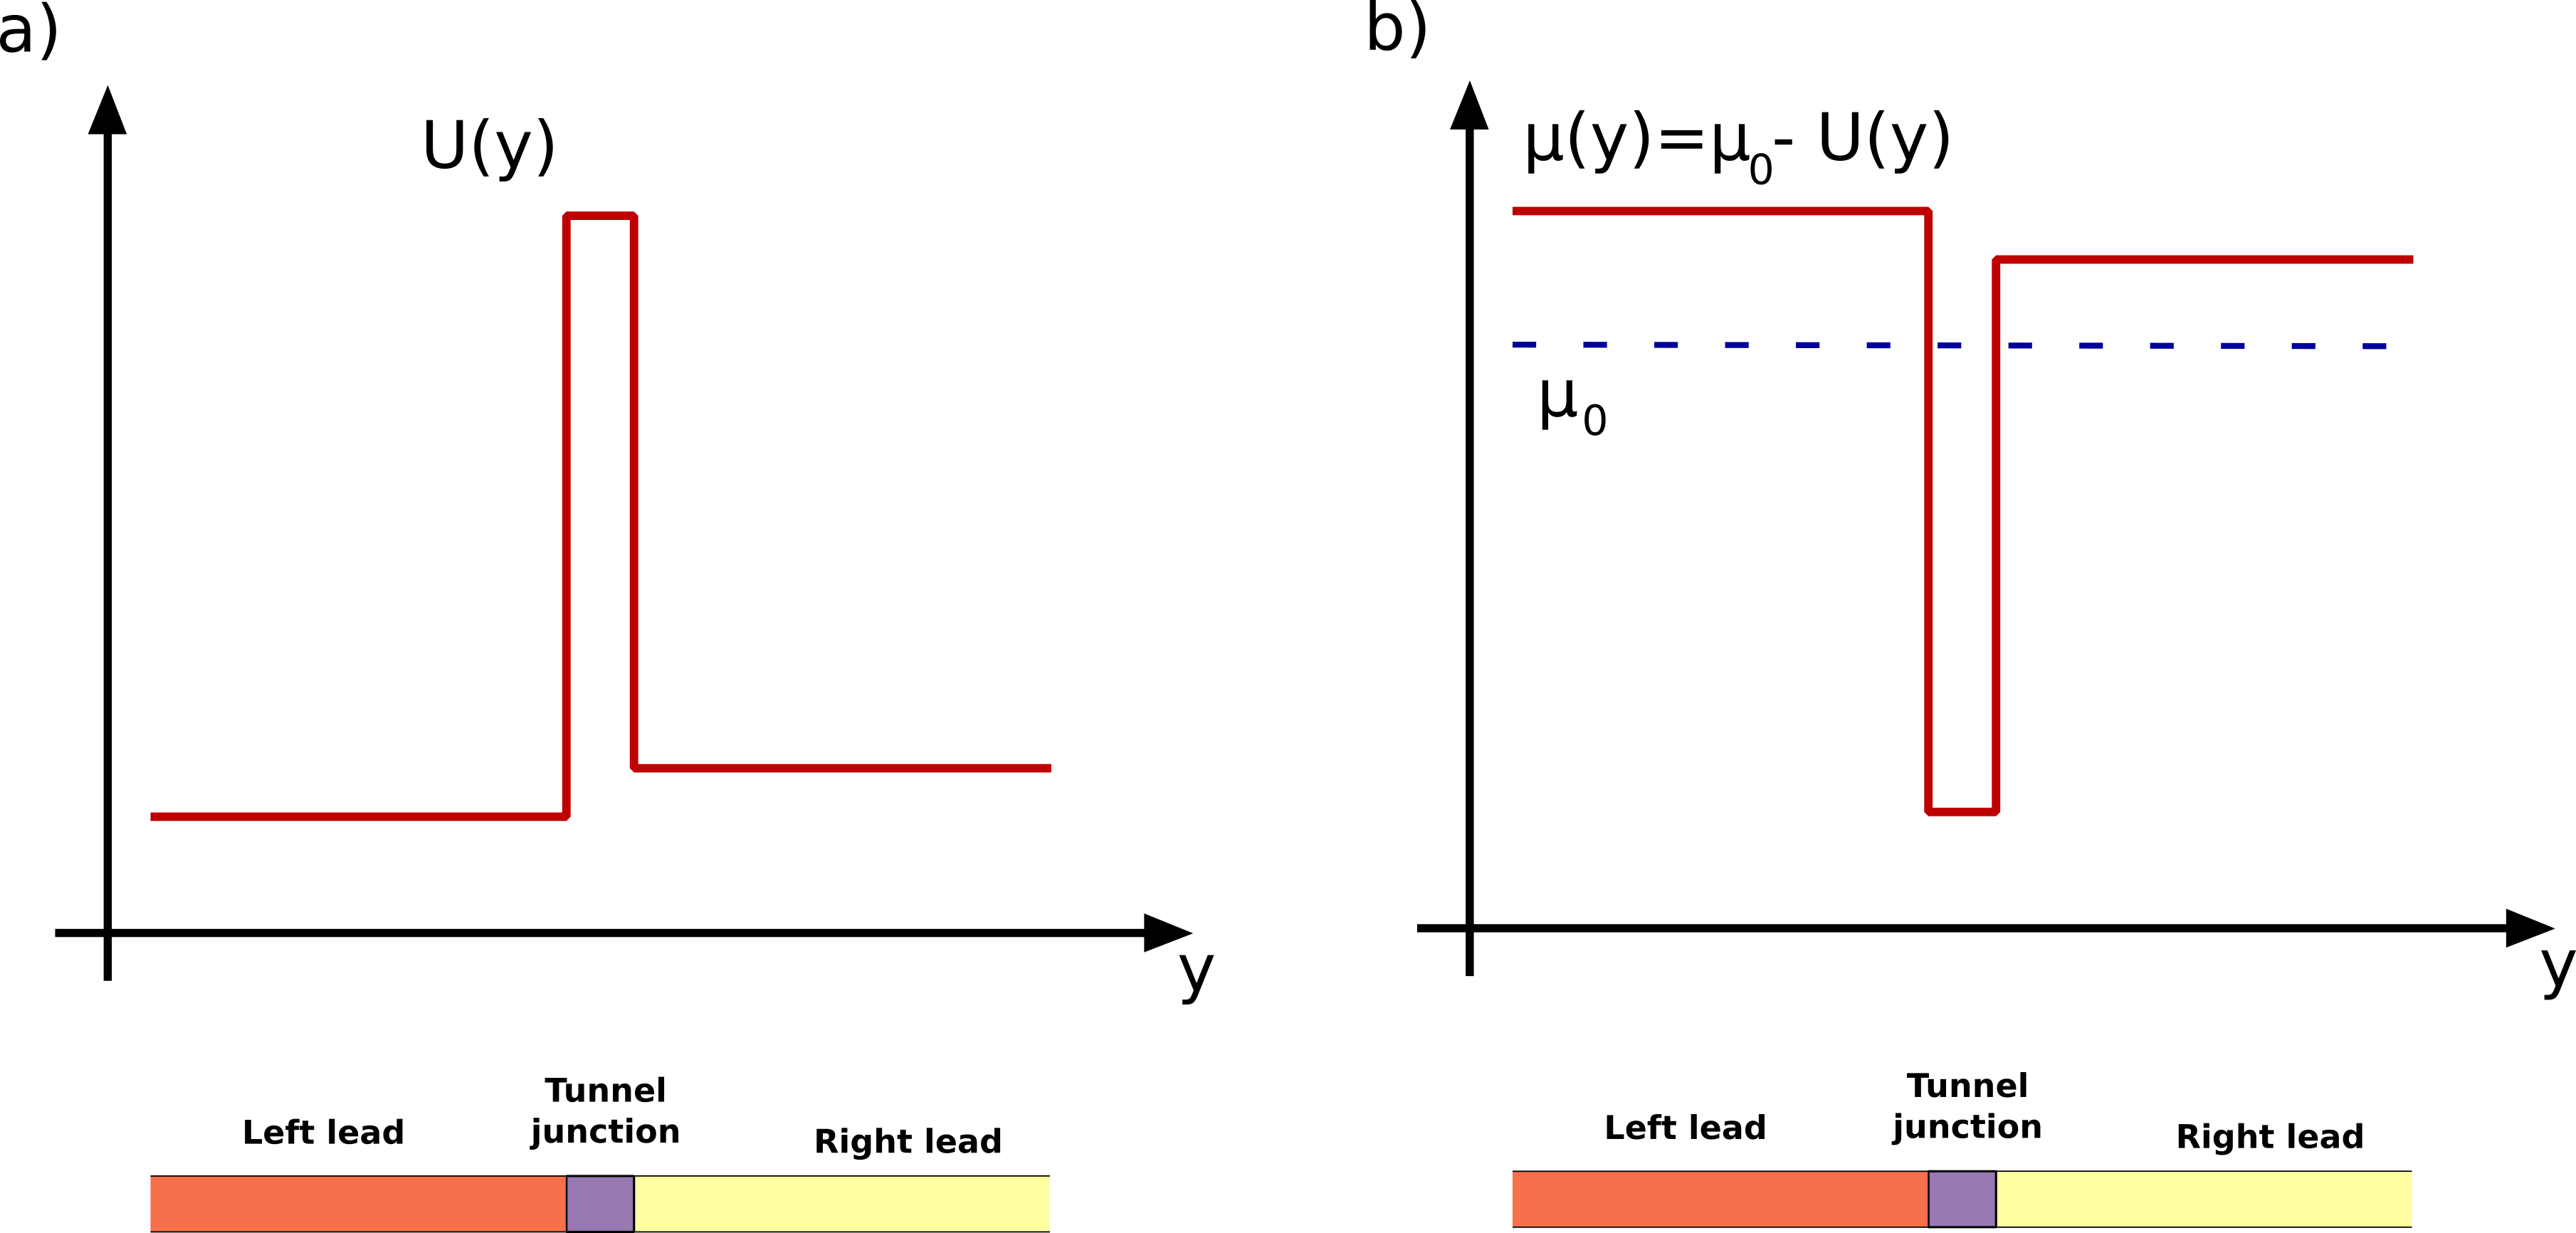
\includegraphics[width=0.8\linewidth]{images/chem_and_ext_potentials}
	\caption{(a) y-profile of external electrical field.  (b) y-profile of effective chemical potential}
	\label{fig:chemandextpotentials}
\end{figure}


Finally, the BdG Hamiltonian for the model reads:
\begin{equation}
\label{full_hamiltonian}
H
=
\br{
	\frac{p^2}{2m}
	-\mu\br{y}
}\tau_z
+
u p \sigma_z \tau_z
+
B\sigma_x	
+
\Delta\tau_{\phi\br{y}}
\end{equation}
with
\begin{equation}
\label{full_hamiltonian_suppl}
	\mu\br{y}
	=
	\begin{cases}
		\mu_L,~~~  -\frac{L}{2}<y\\
		\mu_b,~~ -\frac{L}{2} <y <\frac{L}{2}\\
		\mu_R, ~~~~ \frac{L}{2}< y  
	\end{cases}
	~~~~~~~~
	\phi\br{y}
	=
	\begin{cases}
		\phi_L,&~~~  -\frac{L}{2}<y\\
		\phi_R
		\frac{\frac{L}{2}+y}{L}
		+
		\phi_L
		\frac{\frac{L}{2}-y}{L},
		&~~ -\frac{L}{2} <y <\frac{L}{2}\\
		\phi_R, &~~~~ \frac{L}{2}< y 
	\end{cases}
\end{equation}
with $ L $ being the size of the junction. Note, that the parameters $ B $, $ u $, $ \Delta $ and $ m $ are taken to be constant within all the system.
 
  This setup is close to the one of the models  considered by Oreg et al. in \cite{Oreg_2010} ("\textit{Spatially varying $ \mu $}" section). The difference is in the profile of $ \mu\br{y} $ -- in \cite{Oreg_2010}  there is a step in effective chemical potential, while here this function possesses a well.  
  
 In \cite{Oreg_2010} it's also discussed that the Majorana fermion appear at the inhomogeneity if the relation $ B-\sqrt{\mu^2+\Delta^2} $ is greater than zero at one side of the step in $ \mu\br{y} $ and lesser than zero at another side of it. As will be shown further, this is also relevant to the  system presented here. Note, that if $ B > \left|\Delta\right| $ this condition can always be satisfied by choosing appropriate $ \mu_L $ and $ \mu_R $. 
 
 The model, described by (\ref{full_hamiltonian}) and (\ref{full_hamiltonian_suppl}) possesses a big number of external parameters. Different areas in this parameter space require different approaches and sometimes lead to completely different physics. Here the certain experimentally reasonable constraints are assumed:
  \begin{gather}
 \label{constraints}
 	\mu_L,\mu_R \ll B \sim \Delta \ll mu^2\ll \left|\mu_b\right|
 \end{gather} 

  The experimental justification of this choice is given in the section \textbf{SECTION ABOUT REALIZATION}, while call for it from theoretical point of view will arise further in this chapter.
  


\section{The dispersion of a homogeneous wire}

Before discussing the properties of the junction it's necessary to consider a dispersion of a homogeneous wire modeled with the Hamiltonian (\ref{bulk_Hamiltonian}). Although this can be done exactly, it's instructive to obtain this dependence step by step, starting with a simpler model and adding new terms until the Hamiltonian (\ref{bulk_Hamiltonian}) is restored.

The starting point is the Hamiltonian consisting only of kinetic energy and chemical potential terms: $ H =\frac{ p^2}{2m} - \mu$. It has simple parabolic dispersion presented at fig. \ref{fig:spectrum}(a). When the spin is introduced and spin-orbit coupling term $ up\sigma_z $ is added, the parabola splits in two (fig. \ref{fig:spectrum}(b)), each one corresponding to it's own z-protection of the spin. After introducing a magnetic field with $ B\sigma_x $ term, the gap at the intersection opens (fig. \ref{fig:spectrum}(c)). The next step is introducing the BdG formalism, by adding the multiplier $ \tau_z $ elsewhere except for magnetic field term:  $ 	H = \br{\frac{p^2}{2m} 	-\mu_0 }\tau_z +u p \sigma_z \tau_z + B\sigma_x	 $. This procedure doubles the spectra in a way that each eigenvector with energy $ E $ obtains a partner eigenvector with energy $ -E $, so additional two energy branches appear, being a mirror reflection of  initial dispersion. This is presented at fig. \ref{fig:spectrum}(d), with the dashed lines being BdG partners. The last step is adding the superconducting term $ \Delta\tau_\phi $, which opens the gap where the dashed and the solid lines are intersected (fig. \ref{fig:spectrum}(f)).

As was mentioned before, the dispersion can be found explicitly. As was pointed in \cite{Oreg_2010}, it can be done by squiring the Hamiltonian (\ref{bulk_Hamiltonian}) twice and solving a resulting biquadratic equation, leading to:
\begin{equation}
E^2_{1,2}\br{p}
=
B^2
+
\Delta^2
+
\xi_p^2
+
\br{up}^2
\pm	
2\sqrt{
	B^2 \Delta^2
	+
	B^2\xi_p^2
	+
	\br{up}^2\xi_p^2
}
\end{equation}

with $ \xi_p =\frac{p^2}{2m}-\mu$. This dependence, presented at fig. \ref{fig:spectrum}(f), has two positive and two negative branches, as any BdG dispersion with electron-hole symmetry does. It further discussion only positive branches are considered, if opposite is not mentioned.

\begin{figure}[H]
	\centering
	\includegraphics[width=\linewidth]{images/spectrum}
	\caption{The dispersion of different Hamiltonians:
		 a)  mere kinetic energy and chemical potential: $ H =\frac{ p^2}{2m} - \mu ~~~$
		 b) spin-orbit coupling added: $ 	H = \frac{p^2}{2m}-\mu_0 + u p \sigma_z ~~~$
		 c) magnetic field added: $ 	H = \frac{p^2}{2m} 	-\mu_0  +u p \sigma_z  + B\sigma_x ~~~~~$
		 d) BdG formalism introduced: $ 	H = \br{\frac{p^2}{2m} 	-\mu_0 }\tau_z +u p \sigma_z \tau_z + B\sigma_x	~~~ $
		 e) complete Hamiltonian of homogeneous wire: $ 	H = \br{\frac{p^2}{2m} 	-\mu_0 }\tau_z +u p \sigma_z \tau_z + B\sigma_x	+ \Delta\tau_\phi $.
		 The parameters of the Hamiltonians for plotting are: $ B=0.2 $, $ \Delta=0.3 $, $ u=0.9 $, $ m = 1 $, $ \mu = 0.11 $ 
 }
	\label{fig:spectrum}
\end{figure}

If the constrains (\ref{constraints}) are assumed, the lower branch of this spectra has three minima: one of them is at $ p=0 $ exactly, and two another are at $ p = \pm 2mu $ in the leading order. The last two are not very interesting -- the energy there is approximately equal to $ \Delta $, as it should be due to perturbative introduction of superconducting term. On the contrary, the minimum at $ p=0 $, which is given by\cite{Oreg_2010}:
\begin{gather}
	E_2\br{0}=\abs{g},~~~~g = B -\sqrt{\Delta^2+\mu^2}
\end{gather}
is the most important peculiarity of the spectrum. First, as $\mu\ll B \sim \Delta $, it's the true gap of the spectrum as $  \abs{B^2 -\sqrt{\Delta^2+\mu^2}} \approx  \abs{B-\Delta -\frac{\mu^2}{2\Delta}}\ll\Delta$. Second, the  sign of  $ g $ defines where the wire can or cannot host the Majorana state near some inhomogeneity. Here it's useful to introduce the terminology: if $ g>0 $ the wire is called "toplogical", otherwise it's called "trivial". In \cite{Oreg_2010} and \cite{Lutchyn_2010} it was derived, that the contact of trivial and topological wire hosts a Majorana state. It can also be shown (see section \textbf{ENTER SECTION}), that this state is present on the end of a topological wire and isn't there for a trivial one.

Note, that when two wires are considered, there are two gaps, $ g_{L,R} = B-\sqrt{\Delta^2+\mu_{L,R}^2} $. When the magnetic field $ B $ is close to $ \Delta $, one can change the signs of $ g_{L,R} $ by changing $ \mu_{L,R} $ respectively. 

It's instructive to сlarify the place of $ g_{L,R} $ in the paramter hierarchy of the problem. As $\mu_L \sim \mu_R \ll B\sim \Delta $  and $ g_L=B-\sqrt{\Delta^2+\mu_L^2}<0 $, one can figure out that $\mu_R\sim \mu_L \gtrsim \br{B-\Delta}\br{B+\Delta} $.  Taking that into account and noticing that $ g_{L,R} \approx B-\Delta -\frac{\mu^2}{2\Delta^2}$ and introducing $ \beta=B-\Delta $ one finds $ g_{L,R}\l\lesssim \frac{\beta^2}{\Delta} $, while $ \mu_{L,R} \gtrsim\sqrt{ \beta \Delta} $, so $ \sqrt\ll \mu_{L}, \mu_R $.

\section{Hight and low modes}
\label{sec:high_and_low_modes}

Though the wavefunctions of (\ref{bulk_Hamiltonian}) can be found explicitly, their form is enough complicated to stall any further analysis. However, as the spin-orbit energy is assumed to be the biggest energy scale for a homogeneous wire, one can reduce the Hamiltonian (\ref{bulk_Hamiltonian}) to:
\begin{gather}
\label{short-long_hamiltonian}
	H=\br{\frac{p^2}{2m}+up\sigma_z}\tau_z
\end{gather}

in this problem it's reasonably to assume the low energy limit, as all the Majorana physics should live at the energies of the order of $ g $. Thus the energy term must be omitted in Schroedinger equation, which leads to two types of momenta: $ p_{short} \approx \pm 2mu$ and $ p_{long}\approx 0$ and, respectively two types of wavefunctions: shortwave and longwave ones. The fact that $ p_{long} $ is equal to zero means, that the approximation $(\ref{short-long_hamiltonian})$ is insufficient to describe them. However, to deal with longwave wavefunctions one can omit the quadratic term in (\ref{bulk_Hamiltonian}) and work with linearized Hamiltonian, similar to the ones used in \cite{Oreg_2010} and \cite{Lutchyn_2010}. 
\chapter{Stationary properties} 
\label{chap:stationary_properties}
The stationary properties of the system are defined by it's spectrum. In this chapter the boundary condition is introduced, wavefunctions of the homogeneous wires are obtained, undergap states are investigated and  and the stationary supercurrent is estimated.

\section{Boundary condition}

To obtain the spectrum of the system it's necessary to find the boundary conditions. As the barrier chemical potential  is the biggest energy parameter of the problem, the wave-functions there are defined by the Hamiltonian:
\begin{gather}
\label{barrier_Hamiltonian}
	H(y)
	=
	\br{
		\frac{p^2}{2m}
		+\mu_b
	}\tau_z,  ~~~~~~~~~-\frac{L}{2}<y<\frac{L}{2}
\end{gather} 

as the low energies are the under consideration, in Sroedinger equation the energy term can be omitted, so $ p_b\approx\pm i \sqrt{2m\mu_b} $. One can solve the problem given by (\ref{barrier_Hamiltonian}) and match the values of the wavefunction and it's derivatives on the left and on the right of the barrier to obtain:
\begin{gather}
	\begin{cases}
	\psi_L + b\partial_y\psi_L=t(\psi_R + b\partial_y\psi_R) \\
	\psi_R - b\partial_y\psi_R=t(\psi_L - b\partial_y\psi_L)
	\end{cases}
\end{gather}

here $ \psi_{L,R}=\psi\br{\mp\frac{L}{2}} $, $ b=\br{{2m\mu_b}}^{-\frac{1}{2}} $ --- the penetration depth for the particle inside th barrier and $ t = e^{-\frac{L}{b} }$ --- the tunneling constant assumed to be small: $ t\ll 1 $. This condition reads, that the size of the barrier $ L $ should be  much bigger that the penetration depth $ b $.

This condition is invariant under the combined action $ L\leftrightarrow R $, $ y\to-y $. To simplify the further analysis one can reverce th direction in the left wire and put both ands of the wires from $ y= \frac{L}{2} $ to $ y=0 $. The boundary condition than becomes:
\begin{gather}
\label{bc_transformed}
\begin{cases}
\psi_L - b\partial_y\psi_L=t(\psi_R + b\partial_y\psi_R) \\
\psi_R - b\partial_y\psi_R=t(\psi_L + b\partial_y\psi_L)
\end{cases}
\end{gather}
This transformation is illustrated on the fig \ref{fig:bctransform}. Note

The boundary condition (\ref{bc_transformed}) can be rewritten with introducing the spinor $ \Psi=\br{\psi_L, \psi_R}^T $ and Pauli matrices $ \hat{s}_i $ in LR space:
\begin{gather}
	\br{1-t\hat{s}_x}\Psi-\br{1+t s_x}b\pdy\Psi=0
\end{gather}
since for all $ t\ne 1 $ (recall, that $ t\ll1 $) the matrix is $ 1\pm t\hat{s}_x $ in reversible. Multupliing the last equation by $ \br{1-t\hat{s}_x}/\br{1+t^2} $ one obtain:
\begin{gather}
\label{bc_LR_space}
	\br{1-2\tilde{t}\hat{s}_z-\tilde{b}\pdy}\psi=0
\end{gather}
where $ \tilde{t}=\frac{t}{1+t^2} $, $ \tilde{b} = \frac{1-t^2}{1+t^2}b $. In the leading order on $ t $, which corresponds to the tunneling limit, $ \tilde{t}=t $, $ \tilde{b} = b $.
\begin{figure}[H]
	\centering
	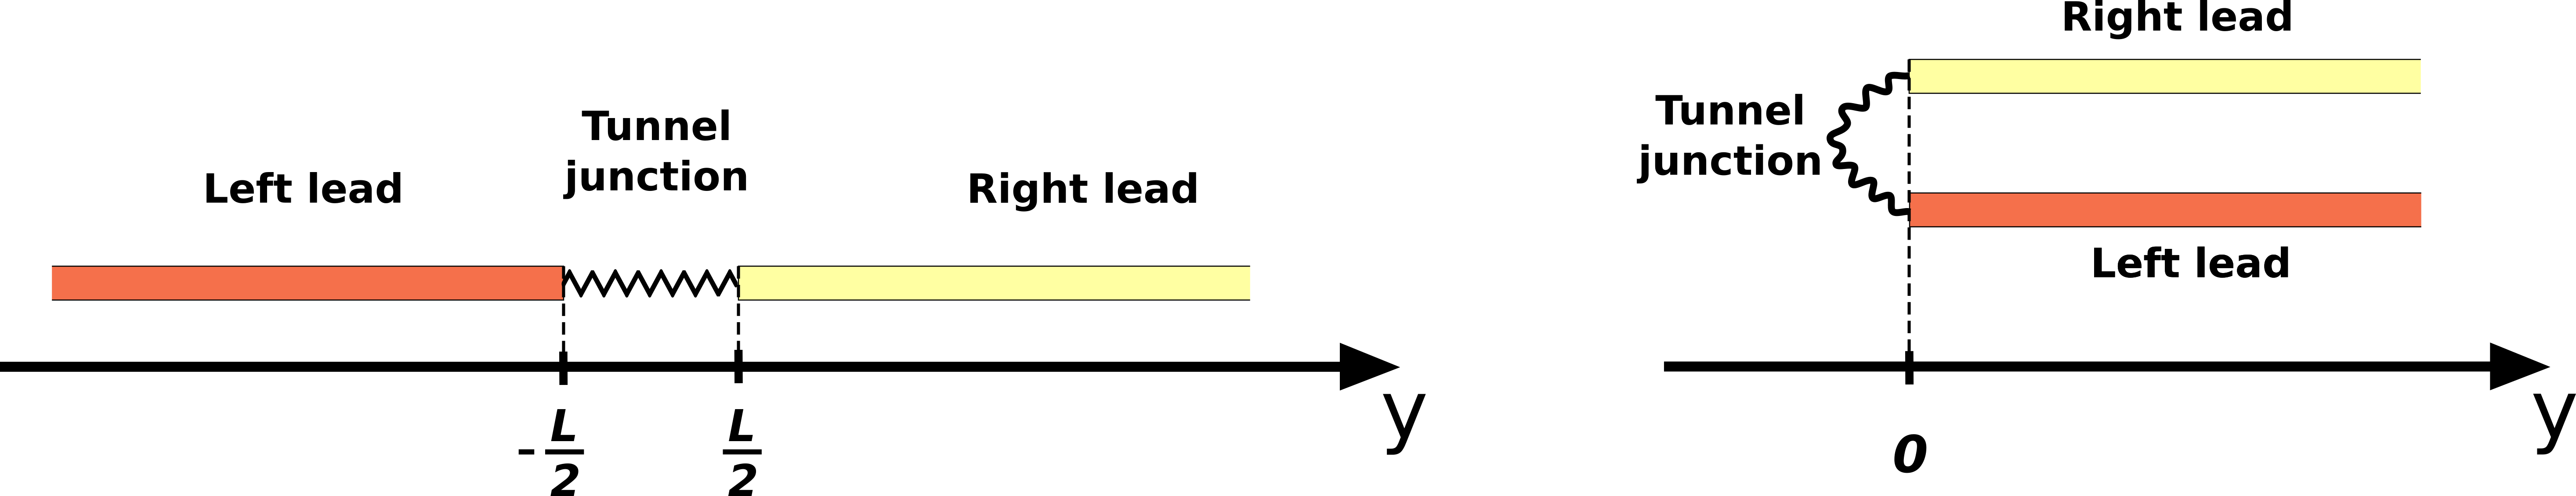
\includegraphics[width=0.9\linewidth]{images/bc_transform}
	\caption{Illustration of switching the direction of left wire}
	\label{fig:bctransform}
\end{figure}

One can argue, that in tunneling limit the second and the third term in (\ref{bc_LR_space}) are much smaller than the first one and should not be taken when the leading order is considered. However, if the second terms is omitted, the leads become efficiently disconnected, and no tunnel effects can be found. The same is true for the third term --- if it's not present, the boundary condition immediately implies $ \Psi\br{0} = 0 $, so the wires become disconnected again.

\section{High momentum modes}  

As was pointed in section \ref{sec:high_and_low_modes}, there are two  shortwave and longwave wavefunctions inside the wire, and the first ones can be described with the Hamiltonian (\ref{short-long_hamiltonian}). However, if one is looking for the localized states, even the longwave modes should be taken decaying. To obtain this, one needs to add a restore superconducting term in (\ref{short-long_hamiltonian}), so the spectrum become gapped and the momenta can get an imaginary part. So, for shortwave modes one should consider a Hamiltonian:
\begin{gather}
\label{high_mods_hamiltonian}
	H=\br{\frac{p^2}{2m}-up\hat{s}_z\sigma_z}\tau_z+\Delta\tau_\phi
\end{gather}
here the multiplier $ \hat{s}_z $ is added in the spin-orbit coupling term, as the direction of the left wire is inverted, so to write a correct Hamiltonian for LR space, one needs to change $ p $ to $ -p $ for the left wire --- which is exactly adding $ -s_z $ multiplier to each momentum.

Denoting $ \eta = \frac{p^2}{2m}-up\hat{s}_z\sigma_z $, one can rewrite (\ref{high_mods_hamiltonian}) as $ H=\eta\tau_z+\Delta\tau_\phi $. As $ \hat{s}_z\sigma_z $ commutes with $ H $ one can treat it as a number, so the dispersion is $ E^2 =\eta^2+\Delta^2 $ (the number corresponding to eigenstate of $ \hat{s}_z $ will be denoted as $ s_z $ while the number, corresponding to the eigenstate of $ \sigma_z $ will be denoted as $ \varsigma_z $). Thus $ \eta=\pm i\sqrt{\Delta^2-E^2} $, as the case $ \abs{E}<\Delta $ is assumed. For momenta\textbf{} one can write the equation:
\begin{gather}
	p^2-2mu s_z \varsigma_z p - 2m \eta =0
\end{gather}
which for shortwave momenta gives $ p_{short}\approx2 mu s_z \varsigma_z + \frac{\eta}{u}s_z\varsigma_z$. Choosing the sign of $ \eta $ in a way, that the wavefunction decays at $ x\to \infty $, one can obtain:
\begin{gather}
\label{short_momentum_decaying}
	p_{short}\approx
	2 mu s_z \varsigma_z 
	+
	i\frac{\sqrt{\Delta^2-E^2}}{u}
\end{gather}


Now the wavefunction can be constructed by putting (\ref{short_momentum_decaying}) into the Schroedinger equation $ \br{\eta\tau_z +\Delta\tau_\phi}\Psi=E\Psi $. The solutions are:
\begin{gather}
	\Psi_{s_z,\varsigma_z}\br{x}
	=
	\begin{pmatrix}
	1
	\\
	e^{i\br{s_z\varsigma_z\gamma+\phi_{s_z}}}
	\end{pmatrix}_{eh}
	e^{2imus_z\varsigma_zx -\frac{\sqrt{\Delta^2-E^2}}{u}x}
	\ket{s_z, \varsigma_z}
\end{gather}
where  $ \ket{s_z, \sigma_z} $ are eigenvectors of matrix $ \hat{s}_z \sigma_z $,  $ \gamma = -\frac{\pi}{2}+\arcsin\frac{E}{\Delta} $ and $ \phi_{1}=\phi_L$, $ \phi_{-1}=-\phi_R $
Thus the longwave part of eqigenstate can be written as:
\begin{gather}
\label{fast_mode_expansion}
	\Psi_{long}
	=
	\sum_{s_z=\pm 1}
	\sum_{\varsigma_z=\pm 1}
	C_{s_z,\varsigma_z}
	\Psi_{s_z,\varsigma_z}\br{x}
\end{gather}
 
  \if 0
\begin{gather}
\begin{pmatrix}
i \hat_z \sigma_z\sqrt{\Delta^2-E^2}-E & \Delta e^{-i\phi_{L,R} s_z} \\
\Delta e^{i\phi_{L,R} s_z} & -i s_z \sigma_z\sqrt{\Delta^2-E^2}-E
\end{pmatrix}
\Psi
=
E\Psi
\end{gather}
\fi


\section{Eliminating longwave modes from boundary condition}
\label{sec:elimintaing_longwave}
As the Majorana mode acts at low energies, it's expected to be predominantly longwave. This argument is in accord with \cite{Oreg_2010} and \cite{Lutchyn_2010}, where the majorana state was an eigenstate of a linearized Hamiltonian, which is relevant only for longwave physics. So, it's reasonable to eliminate the shortwave modes from the problem, reformulating the boundary condition (\ref{short-long_hamiltonian}).

The wave function can be decomposed in shortwave and  longwave  parts: $ \Psi = \Psi_{high}+\Psi_{low} $. inserting it into the(\ref{short-long_hamiltonian}) and using the fact, that $ p_{low}\ll p_{high} \approx 2mu s_z \sigma_z $, one can obtain at the boundary:
\begin{gather}
	\br{1-2t\hat{s}_x}\Psi_{low}+\br{1-2t\hat{s}_x-2ibum\hat{s}_z \sigma_z}\Psi_{high}=0
\end{gather}
Multipluning by the $ \br{1-2t\hat{s}_x}^{-1} $ and eliminating $ {t^2} $ terms, obtain:
\begin{gather}
	\Psi_{low}
	=
	\br{-1+i\zeta\br{1+2t\hat{s}_x}s_z \sigma_z}\Psi_{high}
\end{gather}
with $ \zeta=2bum $.

Now, using the expansion (\ref{fast_mode_expansion}) and renormalizing the coefficients: $ C_{s_z \varsigma_z}\to-\br{1-i\zeta s_z \varsigma_z}C_{s_z \varsigma_z} $ one can rewrite the boundary condition for $ \varsigma_z $ spin component of the wavefunction as:
\begin{gather}
\Psi_{low,\varsigma_z}
=
\br{1+\frac{2i\zeta t\hat{s}_z\sigma_z}{1+i\zeta \hat{s}_z\sigma_z}}
\sum_{s_z=\pm1}
C_{s_z,\varsigma_z}
		\begin{pmatrix}
	1
	\\
	e^{i\br{s_z\varsigma_z\gamma+\phi_{s_z}}}
	\end{pmatrix}_{eh}
	e^{2imus_z\varsigma_zx -\frac{\sqrt{\Delta^2-E^2}}{u}x}
	\ket{s_z, \varsigma_z}
\end{gather}
This can be  multiplied by $ \br{1+\frac{2i\zeta t\hat{s}_z\sigma_z}{1+i\zeta \hat{s}_z\sigma_z}}^{-1} $, which up to a $ t^2 $ correction yields:

\begin{gather}
\label{bc_projection}
	\br{1-\frac{2i\zeta t\hat{s}_z\sigma_z}{1+i\zeta \hat{s}_z\sigma_z}}
	\Psi_{low,\varsigma_z}
	=
	\sum_{s_z=\pm1}
	C_{s_z,\varsigma_z}
			\begin{pmatrix}
	1
	\\
	e^{i\br{s_z\varsigma_z\gamma+\phi_{s_z}}}
	\end{pmatrix}_{eh}
	e^{2imus_z\varsigma_zx -\frac{\sqrt{\Delta^2-E^2}}{u}x}
	\ket{s_z, \varsigma_z}
\end{gather}

For each $ \varsigma_z $ the above equation can be interpreted as the requirement that the l.h.s. 4-vector (in LR- and eh-spaces) lies in the 2d linear space $ L_{2} $ spanned by the the two vectors in the sum in the r.h.s.. This can be reformulated as the requirement that the l.h.s. be orthogonal to the complementary 2d space $ \overline{L}_{2} $. There are two basic vectors $ \overline{\Psi}_{s_z\varsigma_{z}} $ ($ s_z=\pm1 $) spanning $ \overline{L}_{2} $ for each $ \varsigma_z $:
\begin{gather}
	\overline{\Psi}_{s_z\varsigma_{z}}
	=
	\begin{pmatrix}
	1 \\
	-e^{
		i\br{
			s_z\varsigma_z\gamma
			+
			\phi_{s_z}
			}
		}
	\end{pmatrix}
	\ket{s_z,\varsigma_z}
\end{gather}
Thus one needs to multiply (\ref{bc_projection}) by $ \br{\overline{\Psi}_{+\varsigma_{z}},\overline{\Psi}_{-\varsigma_{z}}} $ from the left and, after all evaluating the matrix produt, find the boundary condition on longwave modes in the form:
\begin{gather}
\label{bc_matrix}
\begin{pmatrix}1 & -e^{-i\left(\varsigma_{z}\gamma-\phi_L\right)} & A & -Ae^{-i\left(\varsigma_{z}\gamma-\phi_L\right)}\\
A^{*} & -A^{*}e^{i\left(\varsigma_{z}\gamma+\phi_R\right)} & 1 & -e^{i\left(\varsigma_{z}\gamma+\phi_R\right)}
\end{pmatrix}\Psi_{long, \varsigma_{z}}=0
\end{gather}
here $ A=-\frac{2i\zeta t\varsigma_z}{1+i\zeta\varsigma_z} $ and the elements are ordered as $ \br{Le,Lh,Re,Rh} $.

When studying wavefunctions in superconductors, it is more convenient to work with zero phase $ \phi $. This can be achieved by gauging the phase difference into the boundary condition. Indeed, suppose $ H_{\phi} $ describes a wire with phase $ \phi $. Then, $ H_{\phi}=U_{\phi}^{\dagger}H_{0}U_{\phi} $ with $ U_{\phi}=\mathrm{diag(1,e^{i\phi})_{eh}} $ and the wave functions are also related via unitary rotation $ \psi_{\phi}=U_{\phi}^{\dagger}\tilde{\psi} $. So the transform $ U^{\dagger}=\mathrm{diag}\br{1,e^{-i\phi_L},1,e^{-i\phi_R }}_{Le,Lh,Re,Rh}$  will eliminate all the phases from the wires and put them into boundary condition. Substituting $ \Psi_{low,\varsigma_{z}}=U^{\dagger}\tilde{\Psi} $ into (\ref{bc_matrix}) one arrives at an even simpler boundary condition on the zero-phase function $ \tilde{\Psi} $:
\begin{gather}
\label{bc_matrix_phases}
\begin{pmatrix}1 & -e^{-i\varsigma_{z}\gamma} & A & -Ae^{-i\left(\varsigma_{z}\gamma+\varphi\right)}\\
A^{*} & -A^{*}e^{i\left(\varsigma_{z}\gamma+\varphi\right)} & 1 & -e^{i\varsigma_{z}\gamma}
\end{pmatrix}
\tilde{\Psi}_{long, \varsigma_{z}}=0
\end{gather}
where $ \varphi=\phi_R-\phi_L $. Note, that any physical quantity can depend only on phase difference $ \varphi $,  but not on $ \phi_L $ or $ \phi_R $ separately.

It's also convenient to rewrite it in the form acting on the left and right wire wavefunctions: 

\begin{gather}
\label{bc_matrix_LR}
M_L\tilde{\psi}_{low}^L
+
M_R\tilde{\psi}_{low}^R
=
0
\nonumber
\\
M_L
=
	\begin{pmatrix}
	1 & -e^{-i\sigma_z\gamma}
	\\
	A^* & -A^* e^{i\br{\sigma_z\gamma+\varphi}}
	\end{pmatrix}_{eh}
	\qquad
M_R
=
	\begin{pmatrix}
	A & -A e^{i\br{\sigma_z\gamma+\varphi}}
	\\
1 & -e^{i\sigma_z\gamma}
\end{pmatrix}_{eh}
\qquad	
\end{gather}
This for is especially useful for finding subgap states localized near the barrier.
\section{Low momenta and linearized Hamiltonian}
\label{sec:linearized_hamiltonian}

To utilize boundary condition (\ref{bc_matrix}) or (\ref{bc_matrix_phases}), it's necessary to find low momenta wavefunctions in homogenious wire (this functions constitute $ \psi_{low}$ in (\ref{bc_matrix}) and (\ref{bc_matrix_phases}). For this purpose one can use s linearized version of the Hamiltonian (\ref{bulk_Hamiltonian}), like in \cite{Oreg_2010} and \cite{Lutchyn_2010}:
\begin{gather}
\label{linearized_hamiltonian}
		H
	=
	-\mu \tau_z
	+
	u p \sigma_z \tau_z
	+
	B\sigma_x	
	+
	\Delta\tau_x
\end{gather}
here the zero phase $ \phi $ is assumed and $ \mu $ can be equal $ \mu_L $ or $ \mu_R $ depending on the wire considered. As was mentioned before, the nonzero phase can be restored by using $ U_\phi $ matrix. This hamiltonian is valid only for the right wire. To obtain the solution in the left wire one needs to reverse the sign of $ p $ in (\ref{bulk_Hamiltonian}). Instead of doing so, the unitary transform $ \psi_L=\sigma_x\psi_R $ can be utilized, as for (\ref{bulk_Hamiltonian}) $ H\br{-p}=\sigma_x H\br{p}\sigma_x $.

Remembering, that $ \beta=B-\Delta\ll B, \Delta $, one can	treat this Hamiltonian penetratively, decomposing it as $ H=H_0+V_0$:
\begin{gather}
	H_0=
	u p \sigma_z \tau_z
	+
	\Delta
	\br{\sigma_x	
	+
	\tau_x}
\\
V=-\mu \tau_z+\beta\sigma_x
\end{gather}

As $ H_0 $ commutes with $ \sigma_x\tau_x $, it's convenient to rewrite it in the basis of common eigenstates of $ \sigma_x $ and $ \tau_x $. Denoting them as $ \ket{\sigma_x, \tau_x }$ and arranging the order as $  \br{\ket{+, + },\ket{-, - },\ket{+, - },\ket{-, + }} $ one can rewrite $ H_0+V $ as:
\begin{gather}
	H_0
	=
	\begin{pmatrix}
	2\Delta & up & 0 & 0 \\
	up & -2\Delta & 0 & 0\\
	0 & 0 & 0 & up \\
	0 & 0 & up & 0 
	\end{pmatrix}
	~~~~~~~~
	V
	=
		\begin{pmatrix}
	\beta & 0 & -\mu & 0 \\
	0 & -\beta & 0 & -\mu\\
	-\mu & 0 & \beta & 0 \\
	0 & -\mu & 0 & -\beta 
	\end{pmatrix}
\end{gather}
It's easy to see, subspace $ \mathrm{Span}\br{\ket{+, + },\ket{-, - }} $ require no perturbation to obtain the eigenstates in the leading order. Indeed, diagonalizing the upper subblock of $ H_0 $, one finds, that $ E=\sqrt{\br{2\Delta}^2+\br{up}^2} $. When the low energy states are the objects of interest ($ E\sim g_{L,R} $), one finds, that $ p =\pm\frac{i\Delta}{2u} $ in the leading order, and the corresponding eigenstates are $\ket{+, + }\pm i\ket{-, - } $. If

The another two eigenstates are a little bit more complicated. Diaginalizing  the lower subblock of $ H_0 $, one immediately finds, that $ E=\pm up $. This corrseponds to the fact, that $ H_0 $ is the version of $ H $ with a closed gap $ g $  on lower branch (see fig. \ref{fig:spectrum},(e)), so in the zero order this states cannot form anything localized at all. To find them correctly, one needs to take into account the perturbation $ V $ and solve the secular equation using the following ansatz:
\begin{gather}
	\psi = r_1\ket{+, + }+r_2\ket{-, - }+q_{1}\ket{+, - }+q_{2}\ket{-, + }
\end{gather}
with $ r_i\ll q_j $ for all  pairs $ \br{i,j} $. In the leading order (remeber, that both $ E  $ and $ up $ are of the oreder of $ g_{L,R} $ now) this results to a couple of equations:
\begin{gather}
\begin{cases}
	\br{-E+B-\Delta-\frac{\mu^2}{2\Delta}}q_1+up q_2=0
	\\
	u p q_1 + \br{-E-B+\Delta+\frac{\mu^2}{2\Delta}}q_2 =0
\end{cases}
\end{gather}
recall, that at this precision $ g=B-\Delta-\frac{\mu^2}{2\Delta} $ and find $ E^2=g^2+u^2p^2 $.

For this states the momenta are of the order of $ g/u $, so it's reasonably to name them longwave states. Than the states with momenta $ \pm\frac{i\Delta}{2u} $ will be called mediumwave states.
Now it's time to present this wavefunctions in original BdG basis. The expressions here are relevant only for the right lead and for $ E>0 $. To find the wavefunctions in the left lead, the transform $ \psi_L=\sigma_x\psi_R $ can be used, while for finding the negative enrefu states one can utilize electron-hole transform: $ \psi_{E<0}= \tau_y\sigma_yK\psi_{E>0}$ with $ K $ being a complex conjugation operator.

For $ E>2\Delta $ medium wave states are:
\begin{gather}
	\psi^{out,~in}_{medium}
	\bigg|_{E>2\Delta}
	=
	\begin{pmatrix}
	1
	\\
	\frac{E\mp\sqrt{E^2-4\Delta^2}}{2\Delta}
	\\
	\frac{E\mp\sqrt{E^2-4\Delta^2}}{2\Delta}
	\\
	1
	\end{pmatrix}
	e^\frac{\pm i x\sqrt{E^2-4\Delta^2}}{u}
	\end{gather}
	
	For $ E>2\Delta $ medium wave states are:
	\begin{gather}
	\label{medium_dec_wave_functions}
	\psi^{grow,~dec}_{medium}
	\bigg|_{E<2\Delta}
	=
	\begin{pmatrix}
	1
	\\
	\frac{E\pm i\sqrt{4\Delta^2-E^2}}{2\Delta}
	\\
	\frac{E\pm i\sqrt{4\Delta^2-E^2}}{2\Delta}
	\\
	1
	\end{pmatrix}
	e^\frac{\pm  x\sqrt{4\Delta^2-E^2}}{u}
\end{gather}

For $ E>\abs{g} $ longwave states are:
\begin{gather}
		\psi^{out,~in}_{long}
		\bigg|_{E>g}
=
\begin{pmatrix}
1\\
\frac{E\mp \sqrt{E^2-g^2}}{g}\\
-\frac{E\mp \sqrt{E^2-g^2}}{g}\\
-1
\end{pmatrix}
e^{\pm\frac{ix\sqrt{E^2-g^2}}{u}}
\end{gather}
For $ E<\abs{g} $ longwave states are:
\begin{gather}
	\label{long_dec_wave_functions}
	\psi^{grow,~dec}_{long}
	\bigg|_{E<g}
	=
	\begin{pmatrix}
	1\\
	\frac{E\pm i\sqrt{g^2-E^2}}{g}\\
	-\frac{E\pm i\sqrt{g^2-E^2}}{g}\\
	-1
	\end{pmatrix}
	e^{\pm\frac{x\sqrt{g^2-E^2}}{u}}
\end{gather}

\section{Subgap states}
\label{sec:Subgap_states}

To find the bound states one needs to make two linear combinations (each for it's own wire) of decaying wave functions from (\ref{medium_dec_wave_functions}) and (\ref{long_dec_wave_functions}) at $ x=0 $ and put them into boundary condition (\ref{bc_matrix_LR}). For the right wire they can be taken directly from (\ref{medium_dec_wave_functions}) , (\ref{long_dec_wave_functions}), while for the left wire they should be multiplied by $ \sigma_x $ from the left (see the beginning of section \ref{sec:linearized_hamiltonian}).. These linear combinations can be written as:
\begin{gather}
	\tilde{\psi}_L
	=
	C_{medium}^L
	\sigma_x \psi^{dec}_{medium}
	+
	C_{long}^L
	\sigma_x \psi^{dec}_{L,long}
\qquad
	\tilde{\psi}_R
	=
	C_{medium}^R
	\psi^{dec}_{medium}
	+
	C_{long}^R
	\psi^{dec}_{R,long}
\end{gather}
where $ C_{medium}^L,C_{long}^L, C_{medium}^R,C_{long}^R $ are the undefined coefficients. Note, that the spinor $ \psi^{dec}_{medium} $ is the same for the left and for the right wires.

 Putting these combinations into boundary condition \ref{bc_matrix_LR}, one can obtain four equations for these coefficients. If this system has a solution at energy $ E_0 $, than there is a bound state with this energy. The condition of solvability can be written as:
\begin{gather}
\label{subgap_determinant}
	\det F = 0
\end{gather}
where matrix $ F $ is given by:
\begin{gather}
F
=
	\begin{pmatrix}
	M_L \sigma_x \psi^{dec}_{medium},
	&
	M_L 
	\sigma_x \psi^{dec}_{L,long},
	&
	M_R
	\psi^{dec}_{medium},
	&
	M_R
	\psi^{dec}_{R,long}
	\end{pmatrix}
\end{gather}
As $ E\sim g_{L,R}\ll\Delta $, the mediumwave spinor can be taken in it's low-energy form: 
In the most part of this work the low energy version: $\psi_{medium}^{dec}\approx
\br{
	1,
	- i,
	- i,
	1
}^T
 $
will be used.

For dealing with $ \psi^{dec}_{long} $ it's convenient two introduce to quantities $ \chi_{L,R} $:
\begin{gather}
\cosh\chi_{L,R}
=
\frac{g_{L,R}}{\sqrt{g^2_{L,R}-E^2}}
\qquad
\sinh\chi_{L,R}
=
\frac{E}{\sqrt{g^2_{L,R}-E^2}}
\end{gather}

If $ g>0 $, the corresponding parameter $ \chi $ is real and the monotonously growing with $ E $. For $ g<0 $ the corresponding is complex, but can be parametrized as $ \chi=-\tilde{\chi}+i\pi $ with real and monotonous $\tilde{\chi}  $.

With this parameters the spinors $ \psi_{L\br{R},long}^{dec} $ at $ x=0 $ can be written as:
\begin{gather}
\psi_{L\br{R},long}^{dec}
=
	\begin{pmatrix}
	-\sinh \chi_{L\br{R}} -i
	\\
	-\cosh \chi_{L\br{R}}
	\\
	\cosh \chi_{L\br{R}}
	\\
	\sinh \chi_{L\br{R}} +i
	\end{pmatrix}
\end{gather}
This parametrization completes the toolset used for studying the subgap states.

\subsection{The case of zero tunneling}
Consider first the the equation (\ref{subgap_determinant}) with $ t=0 $. This corresponds to absolutely unpenetrable barrier, orm which is same, to indepensent wires ended with a vacuum. The computation of the determinant in (\ref{subgap_determinant}) becomes a rather easy problem and results in:
\begin{gather}
\label{det_bound_States_zero_t}
	\det F
	\Big|_{t=0}
	=
	-16 \left(i \sinh \left(\chi _L\right)+\cosh \left(\chi _L\right)-1\right) \left(i \sinh \left(\chi _R\right)+\cosh \left(\chi _R\right)-1\right)
\end{gather}

If both $ g_L $, $ g_R $ are negative (triv-triv junction), this determinant cannot be equal to zero at all, as $ \cosh \chi_{L,R} $ are also negative and the real part in each braces always non zero.  If one of $ g_L $, $ g_R $ (triv-top junction), say $ g_R $ there is only one solution at $ E=0 $. If there both $ g_L $, $ g_R $(top-top junction) are positive, there are two solutions at $ E=0 $.

This result proves, that the presence of Majorana mode in a isolated wire is defined only by the sign of $ g $ and justifies the notion of  topology in this system.

\subsection{Small tunneling}
To take into account the tunneling effect one may decompose $ \det F $ in $ t $. Note, that there is no first order in $ t $ due to the structure of boundary condition (\ref{bc_matrix_phases}). The decomposition can be written as:
\begin{gather}
\label{det_f_decomposition}
	\det F
	=
	d_0
	+
	d_2t^2
	+
	\dots
\end{gather}
where $ d_0 $ is given by (\ref{det_bound_States_zero_t}). $ d_2 $ can be computed in a same way, but appears to be  a rather complex formula.  However, in tunneling limit the second correction in (\ref{det_f_decomposition}) should be much smaller than the first one, so the only values of $ E $ that should be considered are the ones with $ d_0 $ is close to zero.

For triv-triv junction there are no such points, so in the tunneling limit there are no bound states for this case.

For triv-top junction there is a solution for $ E=0 $, which corresponds to $ \chi_L=i \pi $, $ \chi_R=0 $. Computing $ d_2 $ for this parameters, one finds that it's exactly zero, so there is no correction to Majorana energy --- as at should be, as it's protected by a particle-hole symmetry.

For top-top junction the situation is more interesting. In that case there are two solutions at $ E=0 $, which should split for nonzero $ t $. Calculating $  $ $ d_2 $ at $ E=0 $ and decomposing $ d_0 $ for small $ E $, one finds:
\begin{gather}
d_0=\frac{16E^2}{g_Rg_L}
\qquad\qquad
	d_2 = -\frac{256t^2\zeta^4}{\br{1+\zeta^2}^2}\cos^2\frac{\phi}{2}
\end{gather}
Using, that $ \zeta=2bum\ll1 $, one can find the energy levels:
\begin{gather}
	E_{1,2}
	=
	\pm
	4t\zeta^2\sqrt{g_Rg_L}\cos\frac{\phi}{2}
\end{gather}
this answer is relevant only if these level are well below the gaps: $ t\zeta^2\sqrt{g_Rg_L}\ll\min\left[g_R,g_L\right] $.
\section{Stationary supercurrent }

\label{sec:stationary_supercurrent}
The stationary supercurrent for a Josephson contact is defined by \cite{Beenakker_three_universal}:

\begin{multline}
\label{beenakker_current}
	I =
	-
	\frac{2e}{\hbar}
	\sum_p
	\tanh\br{\frac{\varepsilon_p}{2k_BT}}
	\frac{d \varepsilon_p}{d\varphi}
	-
	\\
	-
	\frac{4e}{\hbar}
k_BT
	\int\limits_{cont.}d\varepsilon \log
	\left[
		2\cosh\br{\frac{\varepsilon}{2k_BT}}
	\right]
	\frac{d\rho}{d\varphi}
	+
	\frac{2e}{\hbar}
	\frac{d}{d\varphi}
	\int
	d y
		\frac{\abs{\Delta}^2}{\abs{ c}}
\end{multline}
Here $ \epsilon_p $ are the energies of the states localized near the barrier, $ \rho$ is the density of states and $ c\br{\textbf{r}} $ is the interacion constant of the BCS theory, $ \varphi $ is a phase difference, $ k_B $ is a Boltzmann's constant and $ T $ is the temperature.
The first term comes from the discrete spectra and the sum is taken over all states in it, the second term is the current from continuous spectra and the third  term comes from inhomogeneity of the order parameter. As pointed in \cite{Beenakker_three_universal}, despite being generally nonzero, this last term doesn't contribute when step-model functions $ \Delta $ like in (\ref{full_hamiltonian_suppl})  are used.

After ommiting the third term and taking the low temperature limit one rewrites (\ref{beenakker_current}) as:
\begin{gather}
\label{current_low_T}
		I =
		-
	\frac{2e}{\hbar}
	\sum_p
	\frac{d \varepsilon_p}{d\varphi}
	-
	\frac{2e}{\hbar}
	\int\limits_{cont.}\varepsilon d\varepsilon 
	\frac{d\rho}{d\varphi}
\end{gather}

Here the only unknown quantity  is the density of states. As there is a derivative over $ \phi $ taken, one need to find the phase dependent part of $\rho  $ only. It can be done by using the relation between the density of states and the scattering matrix \cite{Akkermans_Avron_Shapiro_scattering_matrix}:
\begin{gather}
\label{smatrix_and_DOS}
	\rho\br{\phi}=\frac{1}{2\pi i}\frac{\partial}{\partial \varepsilon}\log \det S +const.
\end{gather}

As was showed in the section \ref{sec:Subgap_states}, there are no undergap states in triv-top contact except Majorana state. But this state lays exactly on zero energy regardless of the phase difference, so the derivative in the first term of (\ref{current_low_T}) will be zero and no supercurrent from the Majorana state is present.

The scattering matrix can be found with the help of boundary condition (\ref{bc_matrix_phases}) and the results of section (\ref{sec:linearized_hamiltonian}). It's dimension depends of the number of propagating modes at given energy. In this section only the triv.-top. contact will be considered, while the scattering matrices and DOS for other types of contacts will be given in the appendix.

The process of building s-matrix is the following. Firstly, it's necessary to consider an energy and all the propagating  wavefunctions at this energy. Among them there are wave functions, localized near the barrier ($ \mathrm{Im}p>0 $), propagating towards the barrier ($  p<0 $), and propagating from the barrier ($ p<0 $). Let's denote these  three sets as $ X_{local} $, $ X_{in}  $ and $ X_{out} $. Each wavefunction $ \psi_i $ may contribute with it's own coefficient $ C_i $ --- denote the vectors of the coefficients  $ \vec{Y}_{local} $, $ \vec{Y}_{in}  $ and $ \vec{Y}_{out} $ . The s-matrix connects the coefficients from $ \vec{Y}_{in}  $ to $ \vec{Y}_{out} $ in a following wav:
\begin{gather}
	\vec{Y}_{out} = \hat{S}\vec{Y}_{in}
\end{gather}
to find a row of $ \hat{S} $, one should be taken equal to unity, than take  the functions from $ X_{local} $, $ X_{out} $ and one chosen function $ \Psi_{in,chosen} $ from $ X_{in} $ and make the linear combination of the form: $\Upsilon =\psi^{in}_{chosen} + c^{out}_1\Psi^{out}_1+c^{out}_2\Psi^{out}_2+...+c^{out}_1\Psi^{out}_1+c^{local}_2]Psi^{local}_2+... $. The one needs to act with the matrix $ \ref{bc_matrix_phases} $ on $ \Upsilon $ and obtain a set of equations for the coeffixints $ {c^{in}_i} $ and $ {c^{local}_i} $. This system should be solved,and the resulting coefficients ${c^{in}_i}  $ shold form a row in $ \hat{S} $, corresponding to $ \Psi_{in,chosen} $ . To construct the entire matrix $ \hat{S} $, one should repeat this procedure for every function $ \Psi_{in,chosen} $ in $ X_{in} $.

The coefficients of $ \hat{S} $ generally depend on the normalization of the wavefunctions in $ X_{local} $, $ X_{in}  $ and $ X_{out} $. To make the formula (\ref{smatrix_and_DOS}) valid, one must take the functions from $ X_{local} $ normalized to unity and the functions from $ X_{in}  $, $ X_{out}$ normalized to a flux\cite{Akkermans_Avron_Shapiro_scattering_matrix}: $ \bra{\psi_{in,out}}v \ket{\psi_{in,out}} $ with $ v $ for our problem being $ v=u\sigma_z\tau_z $.

Here some additional parameters will be used. When the given wavefunction is localized ($ e<g $), $ \theta $-parametrization is used:

\begin{gather}
\theta_{L,R}:~~~\sin \theta_{L,R} =\frac{E}{g_{L,R}},~~~\cos \theta_{L,R}>0
\end{gather}
this parametrization is useful for both trivial and topological wires. When the wavefunction propagates ($ E>g $), the $ \eta $- ot $ \kappa $-parametrization is used, depending on the sign of $ g $:
\begin{gather}
	\eta_R: ~~~\cosh\eta_R = \frac{E}{g_R},~~~\sinh \eta_R >0
	~~~~~~~~
	\kappa_L: ~~~ \cosh\kappa_L= \frac{E}{\abs{g_{L}}},~~~\sinh \kappa_L>0
\end{gather}
The way to memorize it is that the $ \eta $ is used for a topological wire, whether the $ \kappa $ is used for a trivial wire. All the parameters $ \theta_{L,R}  $,  $\kappa_L $ and $ \eta_R $ are always real and positive when used.

As the dimension of  s-matrix depends on the number of propagating modes, and thus on the energy, it's necessary to investigate different energy ranges separately 
\subsection{$ E $ \hspace{0pt} between $ \abs{g_L} $ and $ g_R $}
	
Recall, that the trivial wire is placed on the left of the barrier while the topological wire is on the right of it. There are two slightly distinct cases, which differ by relation between $ g_L $ and $ g_R $.
\subsubsection{The case $ \abs{g_L} > g_R $}

For $ g_R<E<\abs{g_L} $ there is only one state in $ X_{in} $, so the s-matrix has the dimension 1, so it's determinant coincides with it's only matrix element, which reads:

\subsubsection{The case $ \abs{g_L} < g_R $}
When $ \abs{g_L}<E<g_R $ there is also only one state in $ X_{in} $ and the s-matrix is:


\subsection{$ E $ \hspace{0pt} is greater than both $ \abs{g_L} $ and $ g_R $}

Here there are two states in $ X_in $ -- one in the right wire and one in the left. Thus the s-matrix has the dimension equal to two and reads, up to a $ t^2 $ order:

\chapter{Ionization}
\label{chap:ionization}

In this chapter the model presented before is modified by introducing a small oscillating  external voltage. This perturbation allows the Majorana state to excite into continuum --- the process we will call ionization. The main goal here is to find the ionization rate when the typical size of the photon is much smaller than the spectrum gap.  Only regime with $ \abs{g_L}\ll g_R $ is considered --- this significantly simplifies the calculation, but still exhibits non-trivial physics with a number of different subregimes. 

\section{Introducing the perturbation}

 The perturbation is introduced as an oscillating	 voltage applied to the junction. This alters the Hamiltonian (\ref{full_hamiltonian}) in two ways --- by the modification of the chemical potentials $ \mu_L, \mu_R $ and by making the superconducting phase difference $ \varphi=\phi_R-\phi_L $ time dependent. The second effect is governed by the Josephson relation:
\begin{gather}
	U\br{\tau}
	=
	\frac{\hbar}{2e}
	\frac{\partial\varphi\br{\tau}}{\partial \tau}
\end{gather}

The ionization voltage is assumed to be small compared to other energy parameters, and this smallness is present in both effects. However, if the frequency $ \omega $ of voltage is also small, the perturbation in $ \Delta $ induced by the second effect will have additional big multiplier $ \frac{\Delta}{\omega} $ and will dominate the perturbation in $ \mu $. In this chapter only this regime is considered.

Time dependence of phase difference is introduced as:
\begin{gather}
	\varphi\br{\tau}=\varphi_0+\alpha\cos\omega \tau
\end{gather}
where $ \varphi_0 $ is an initial time independent phase difference and $ \alpha\ll1 $ is the amplitude of phase oscillations.

As was shown in section  \ref{sec:elimintaing_long-wave}, there is a gauge transform $ U_\phi $, which  redistributes the phase difference between the wires, so the phase in a given wire can have any value. This ambiguity just reflects a  fact, that only phase difference $ \varphi $ is an observable quantity, but not the phases $ \phi_L $, $ \phi_R $ separately. However, when treating the time dependent  phase difference this gauge transform also becomes time-dependent. After its application the additional term $ \dot{U}_{\phi\br{\tau}}U_{\phi\br{\tau}}^\dagger \propto \dot{\phi}\br{\tau}$ will appear, but, as $ \omega $ is small, it can be neglected. The corresponding condition on $ \omega $ is established in section \ref{subsec: adiabaticity condition}. 

As the term $ \dot{U}_{\phi\br{\tau}}U_{\phi\br{\tau}}^\dagger \propto \dot{\phi}\br{\tau}$ is negligible, we again can gauge all the phase difference into the boundary condition. Now the boundary condition is time-dependent. It's not very convenient, and to avoid dealing with it we reformulate the problem in terms  of tunnel Hamiltonian, which allow us to treat both tunneling and time dependence simultaneously via perturbation theory.


\if 0

We introduce the time-dependent phases as: $ \phi_L=-\frac{\varphi_0}{2}-\frac{\alpha}{2}\cos \omega t $, $ \phi_R=-\phi_L=\frac{\varphi_0}{2}+\frac{\alpha}{2}\cos \omega t $. Thus the superconducting terms in the wire Hamiltonians alter: $ \Delta_{\pm\frac{\varphi}{2}} \to\Delta_{\pm\frac{\varphi}{2}\pm \frac{\alpha}{2}\cos \omega t} $. Decomposing them in small $ \alpha $ one can explicitly write the perturbation and try to compute the ionization rate. However this way appears to be quite difficult as the overlaps of all the states 
present in both wires and at first it seems that the Majorana states has too much ways to ionize. To avoid this difficulty, the tunnel Hamiltonian approach is used.

\fi

\section{Tunnel Hamiltonian approach}
\label{sec:tunnel_hamiltonian}
The main idea of this method is to hide all the time dependence and the tunnel effect in one single operator. To do so we need to rewrite the Hamiltonian as $ H=H_L+H_R+H_T $, where $ H_{L,R} $ are the Hamiltonians of the left and right wire without any contact (corresponding to zero tunneling: $ t=0 $), and $H_T  $ is a tunnel Hamiltonian both containing the time dependence and mixing the wavefunctions from different wires. 
Here the following notation is used: the Hamiltonians $ H_L $, $ H_R $ and $ H_T $ are 8x8 matrices in combined Nambu-Gorkov and LR-space. In LR-space they have the following form:
\begin{gather}
\label{tunnel_Hamiltonian_formalizm}
	H_L
	=
	\begin{pmatrix}
	h_L & 0 \\
	0 & 0
	\end{pmatrix}_{LR}
	\quad
	H_R
=
\begin{pmatrix}
0 & 0 \\
0 & h_R
\end{pmatrix}_{LR}
\quad
	H_T
=
\begin{pmatrix}
0 & h_{LR} \\
h_{RL} & 0
\end{pmatrix}_{LR}	
\end{gather}
The Hamiltonians $ h_L $ and $ h_R $ eventually coinside with (\ref{bulk_Hamiltonian}) with zero boundary condition. The Hamiltonian $ h_{LR}=h_{Rl}^\dagger $ in unknown --- the goal is to make it in a way the corrections for the wavefunctions are restored . This wavefunctions and their  first tunneling corrections are listed in  appendix \ref{app:wavefunctions_with_corrections}.

The derivation of tunnel Hamiltonian matrix elements is presented in appendix \ref{app:tunnel}. Using the notation  $ \big|\gamma_{0}\,\big> $ for Majorana state and $ \big|\varepsilon,L_{0}\,\big> $, $ \big|\varepsilon,R_{0}\,\big> $ for continuous spectra, we have the following:
\begin{gather}
H_T=
\left(e^{i\frac{\varphi}{2}}+e^{-i\frac{\varphi}{2}}\right)
\tilde{H}_{T}
=
\left(e^{i\frac{\varphi}{2}}+e^{-i\frac{\varphi}{2}}\right)
\begin{pmatrix}
0 & \tilde{h}_{LR} \\
\tilde{h}_{RL} & 0
\end{pmatrix}
\\
\label{tunnel_matrix_elements_maj-cont}
	\big<\gamma_{0}\,\big|\tilde{h}_{RL}\big|E,L_{0}\,\big>
	=
	4\sqrt{ug_{R}}
	t\zeta^{2}
	f\br{\frac{E}{\abs{g_L}}}
	\\
	\label{tunnel_matrix_elements_cont-cont}
	\big<\epsilon,R_{0}\,\big|\tilde{h}_{RL}\big|E,L_{0}\,\big>
	=
	-16u\zeta^{2}t
	f\br{\frac{E}{\abs{g_L}}}
	f\br{\frac{\varepsilon}{g_R}}
\end{gather}
where $ f\br{x}=\sqrt{x^2-1}\br{x+\sqrt{x^2-1}} $. 

 The fact, that all energy dependences here are described by a single function $ f\br{x} $ insinuates that maybe it's possible to make this calculations in a more beautiful way.

\section{Ionization rate for $ g_R\gg\abs{g_L} $}


\subsection{Time dependence of perturbation}

To obtain the ionization rate one should treat $ H_T $ as perturbation. For unperturbed system, described with $ H_0=H_R+H_L $, the electrons cannot get from wire to another, but $ H_T $ allows these processes, so the ionization can be described as a set of jumps from right to left wire (see fig. \ref{fig:tunneling}).

\begin{figure}[H]
	\centering
	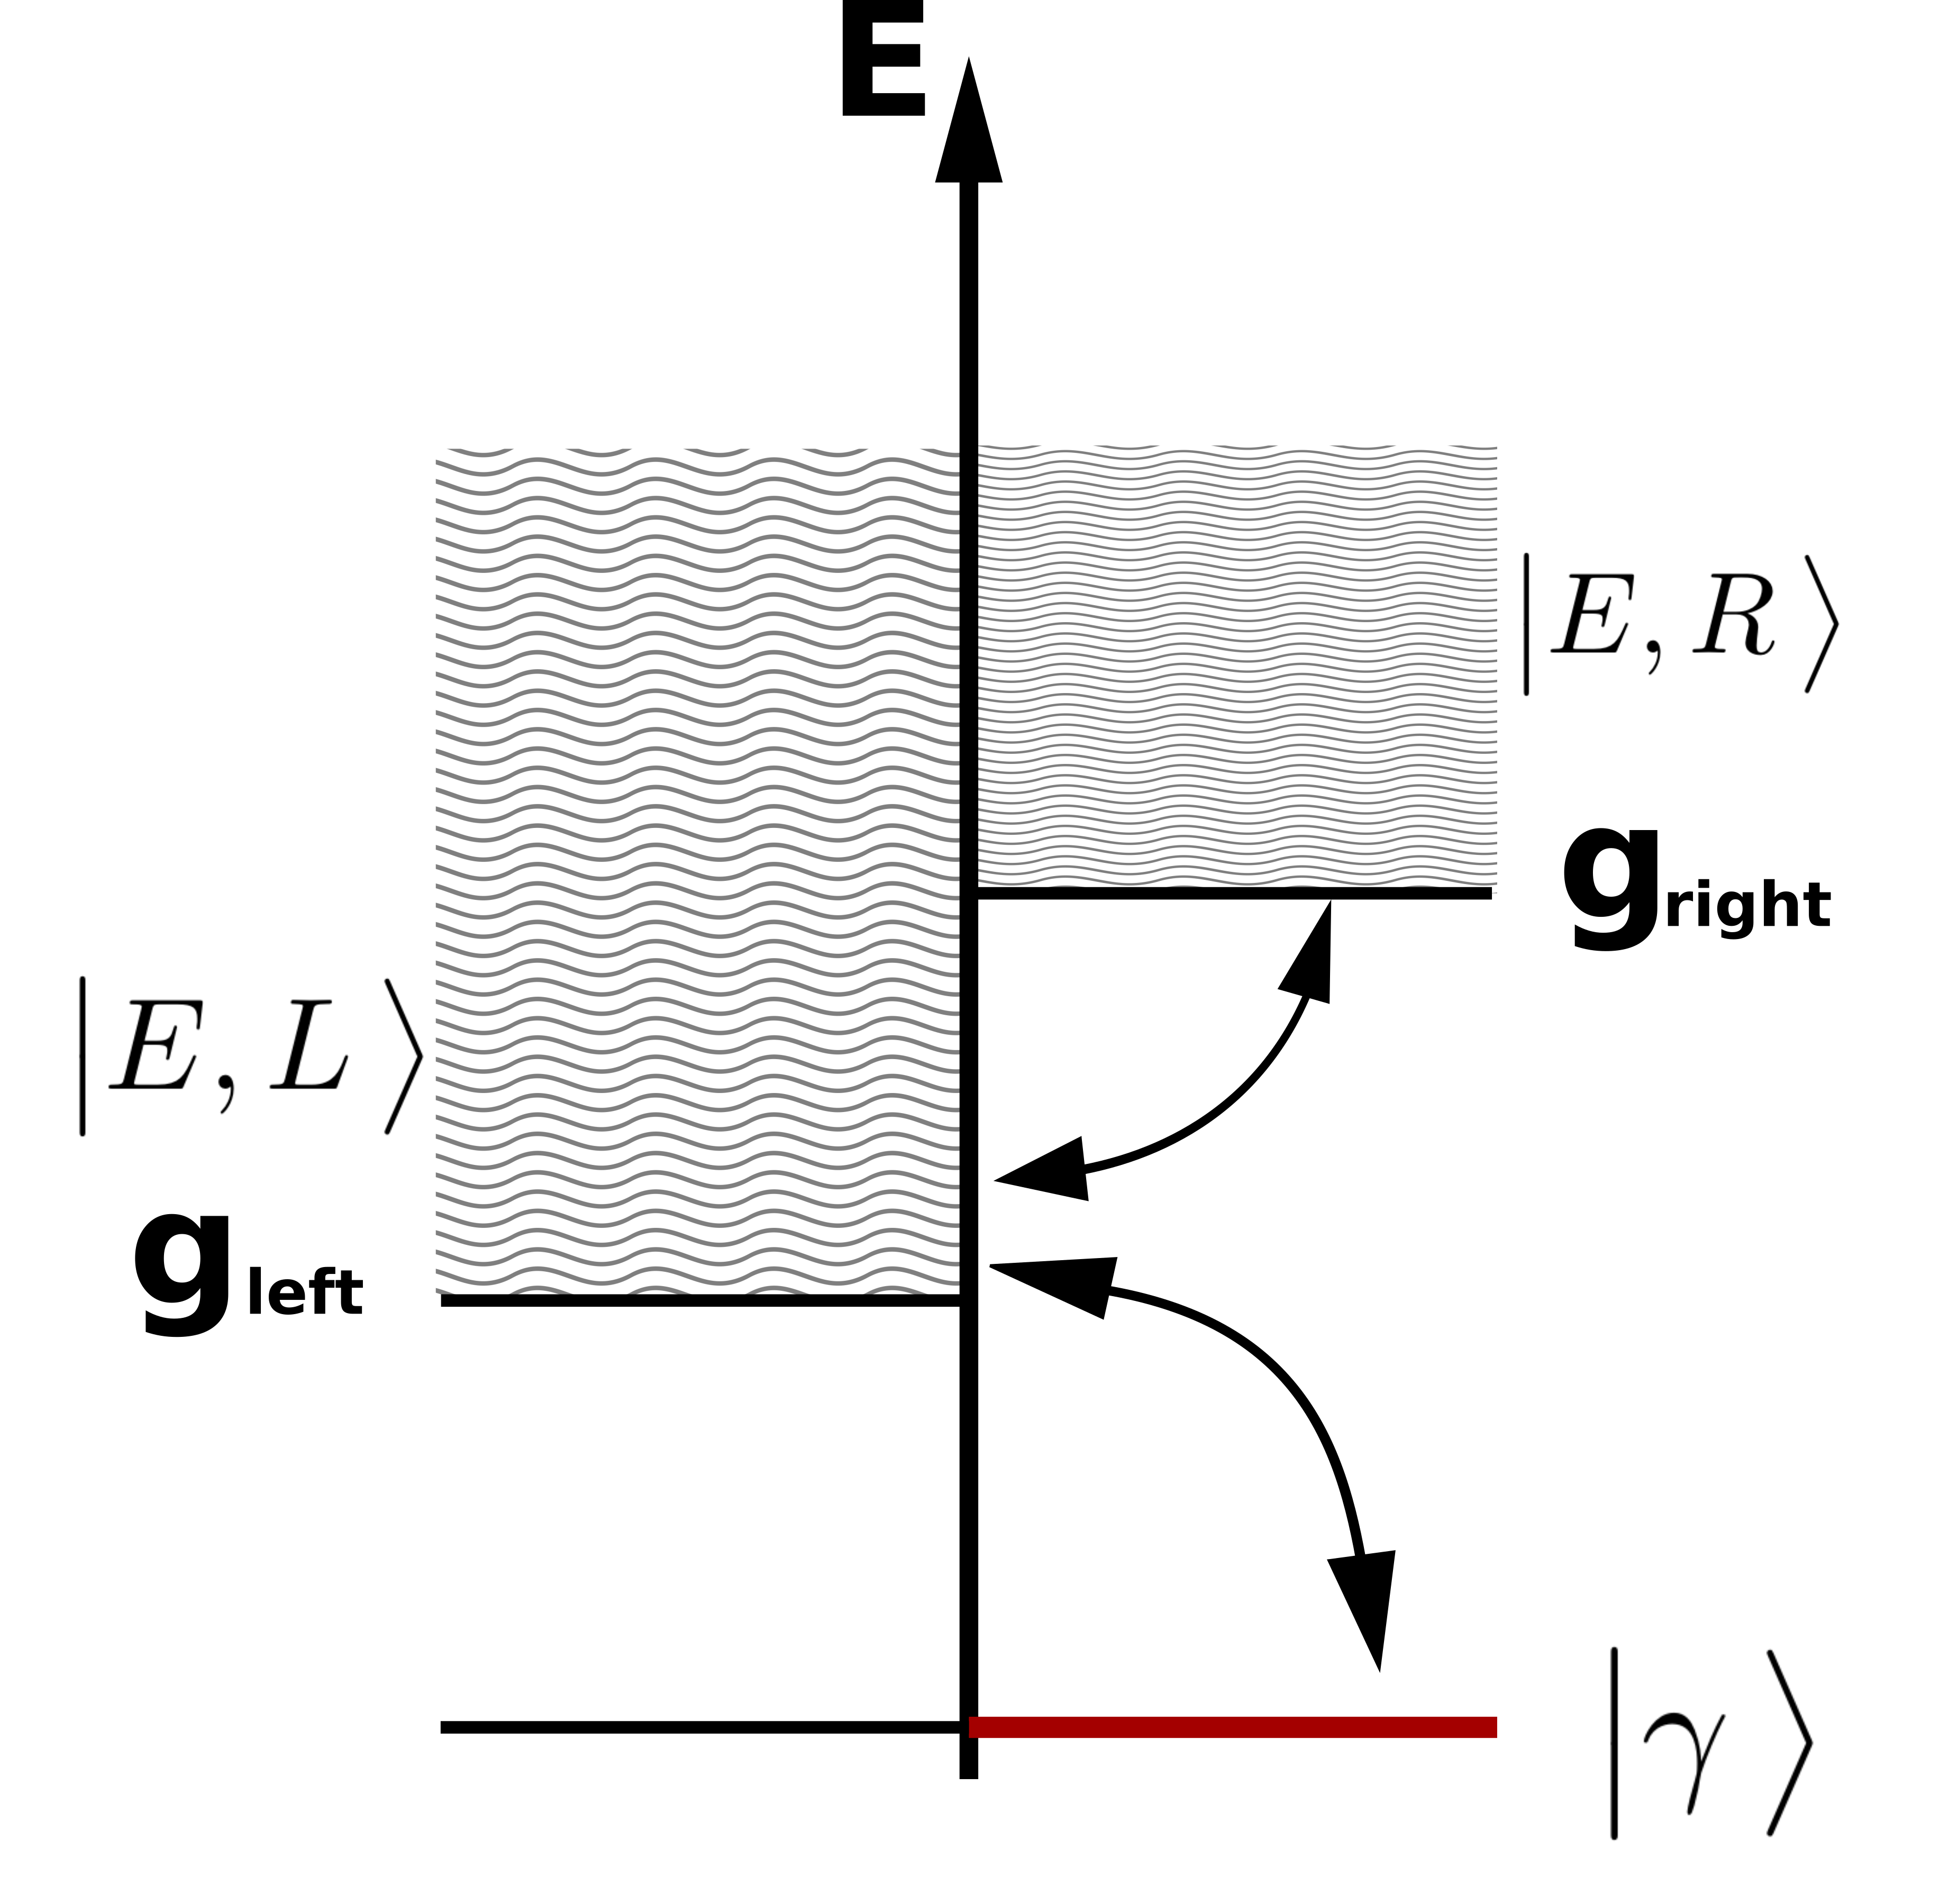
\includegraphics[width=0.65\linewidth]{images/tunneling}
	\caption{Ionization processes in terms of tunnel Hamiltonian}
	\label{fig:tunneling}
\end{figure}

The approach to multiphoton ionization is described in Appendix \ref{app:multiphoton ionization}.  The first step is to decompose the  perturbation in Fourier series in frequencies. From  (\ref{tunnel_matrix_elements_maj-cont}) one finds, that $ H_T\propto\cos\frac{\varphi\br{\tau}}{2} $ with $ \varphi\br{\tau}=\varphi_{0}+\alpha\cos\omega \tau $. Using $ \alpha\ll1 $, we write:
\begin{multline}
	e^{\frac{i\varphi\br{\tau}}{2}}+e^{-\frac{i\varphi\br{\tau}}{2}}\simeq e^{i\frac{\varphi_{0}}{2}}\sum_{n}\frac{(i\alpha)^{n}}{2^{n}n!}(e^{in\omega \tau}+e^{-in\omega \tau})+c.c=
	\\
	=\sum_{n}\frac{\alpha{}^{n}}{2^{2n-1}n!}(e^{in\omega \tau}+e^{-in\omega \tau})\cos\left(\frac{\varphi_{0}}{2}+n\frac{\pi}{2}\right)
\end{multline}
so:
\begin{gather}
\label{tunnel_hamiltonian_harmonics}
	H_{T}=
	\sum_n
	H_{T,n}
	\br{
	e^{in\omega\tau }
	+
	e^{-in\omega\tau }
	},
	\qquad
	H_{T,n}
	\approx
	\sum_{n}	
	\frac
	{\alpha^{n}}
	{2^{2n-1}n!}
	\cos\left(\frac{\varphi_{0}}{2}+n\frac{\pi}{2}\right)
	\tilde{H}_{T}
\end{gather}
The same decomposition is valid for $ LR $ matrix elements of $ H_T $:
\begin{gather}
h_{LR}=
\sum_n
h_{LR,n}
\br{
	e^{in\omega\tau }
	+
	e^{-in\omega\tau }
},
\qquad
h_{LR,n}
\approx
\sum_{n}	
\frac
{\alpha^{n}}
{2^{2n-1}n!}
\cos\left(\frac{\varphi_{0}}{2}+n\frac{\pi}{2}\right)
\tilde{h}_{LR}
\end{gather}
Then the rate is given by (see Appendix \ref{app:multiphoton ionization}):
\begin{gather}
\label{ionization_key}
\mathcal{I}
\sim
\frac{|\langle\mathcal{E}|w_{\mathcal{E}}|\gamma\rangle|^{2}}{N_L(\mathcal{E})},
\qquad
w_{\mathcal{E}}(E)
=
\sum_{\{n_{i}\}:\mathcal{E}}H_{T,n_{N}}\prod_{j=1}^{N-1}G_{0}\left(E+\sum_{s=1}^{j}\omega_{n_{s}}\right)H_{T,n_{j}}
\end{gather}
here sum is taken over all sets $ \{n_i\}:\mathcal{E} $ so that $ \sum_{i} \omega_{n_i}=\mathcal{E}=\min[g_R, \abs{g_L}]$. Each term in sum (\ref{ionization_key}) corresponds to some way (i.e. trajectory) to absorb photons with energies $ \omega_{n_i} $, such that the total absorbed energy is equal to spectrum gap.

For unperturbed Green function we take a notaion:
\begin{gather}
	G_0\br{E}
	=
	\begin{pmatrix}
	G_L\br{E} & 0 \\
	0 & G_R\br{E}
	\end{pmatrix}_{LR}.
\end{gather}

In this section the focus is on the case where the topological gap is much larger than the trivial one: $ \abs{g_L}\ll g_R $. Then the right continuum has high energies and does not participate in the ionization process. Indeed,
\begin{gather}
	h_{LR} G_R\br{\epsilon} h_{RL}
	=
	\frac{h_{LR}|\gamma\rangle\langle\gamma|h_{RL}}{\epsilon}
	+
	\intop_{|E|>g_{R}}
	\frac{h_{LR}|E,R_0\rangle\langle E,R_0|h_{RL}}{\epsilon-E}\frac{dE}{N_{R}(E)}
\end{gather}
So, when $ g_{R}\gg\epsilon\sim \abs{g_L} $, the second term is small and can be neglected. Then, the product $ \dots h_{RL}G_L\br{E}h_{LR}G_R\br{E}h_{RL}\dots $ factorizes into individual factors, which we denote as $ J_{nm}\br{E}\equiv\langle\gamma|h_{RL,n}G_L\br{E}h_{LR,m}|\gamma\rangle $.

\subsection{Factorizing $ w_\mathcal{E} $}
\label{sect:factorizeing_w}

As each entry in the sum within $ w_{\mathcal{E}} $ has the form $ \dots h_{lR}G_R\br{E}h_{RL}G_L\br{E}h_{LR}\dots $, we have:
\begin{gather}
	\sqrt{\mathcal{I}}\propto
	\sum_N \sum_{\{n_i\}_M^N}
	J_{n_1 n_{2}}
	J_{n_3 n_{4}}
	\cdots
	J_{n_{N-1}n_{N}}
\end{gather}
Here $ N $ has the meaning of total number of absorbed photons, $ M $ is the integer closest to $ \frac{\abs{g_L}}{\omega }$ , and the second sum is taken over all sets $ \{n_i\}_M^N $ of $ N $ items such that $ \sum_{i=1}^N n_{i} = M$. We set, the number $ N $ to be even, hiding the last photon into unimportant prefactor.

 The $ n $,$ m $-dependence factors out:
\begin{gather}
J_{nm}\br{E}
=
	\frac{\alpha^{n+m}}
	{2^{2\br{n+m}-2}n!m!}
	\cos\left(\frac{\varphi_{0}}{2}+n\frac{\pi}{2}\right)
	\cos\left(\frac{\varphi_{0}}{2}+m\frac{\pi}{2}\right)
	Q_0\br{E}
\end{gather}
\begin{gather}
	Q_{0}(E)
	=
	\langle\gamma|\tilde{h}_{RL}G_L(E)\tilde{h}_{LR}|\gamma\rangle
	\equiv
	\intop_{cont.}\frac{|\langle\gamma|\tilde{h}_{LR}|\epsilon\rangle|^{2}}{E-\epsilon}\frac{d\epsilon}{N_L(\epsilon)}
\end{gather}

On each ionization step  the particle can move to the state with energy $ E $ or $ -E $, so:
\begin{gather}
	Q_{0}(E)
	=
	2E\intop_{|g_{L}|}^{\infty}\frac{|\langle\gamma|\tilde{h}_{RL}|\epsilon\rangle|^{2}}{E^{2}-\epsilon^{2}}\frac{d\epsilon}{N_L(\epsilon)}
\end{gather}
recalling (\ref{tunnel_matrix_elements_maj-cont}), we obtain:
\begin{gather}
\label{ionization_brick}
		Q_{0}(E)
		=
		ET\frac{\left[-1+\sqrt{1-\lambda^{2}}\right]}{\lambda^{2}}
\end{gather}
where $ \lambda = \frac{E}{\abs{g_L}} $, $ T=\frac{g_R\br{\zeta^2t}^2}{\abs{g_L}} $. We consider $ T\ll 1$, so the systems remains in a strong tunneling limit.

Thus, the elementary block  in our product for small enough $ n $ becomes:
\begin{gather}
	\frac{J_{nm}}{E+n\omega}
	\approx
	\frac{J_{nm}}{E}
	=
	\br{\frac{\alpha}{4}}^{n+m}
	B_n B_m T
	\frac{-1+\sqrt{1-\lambda^2}}{\lambda^2}
\end{gather}
where
\begin{gather}
	B_n=
	\frac{2}{n!}\cos\br{\frac{\phi_0}{2}+\frac{\pi n}{2}}
\end{gather}

The prefactor $  \br{\alpha/4}^{n+m} $ yields $ (\alpha/4)^{\mathcal{E}/\omega} $ for any trajectory and therefore do not affect summation and optimization. Thus one has $ B_{n}B_{m}T\frac{-1+\sqrt{1-\lambda^{2}}}{\lambda^{2}} $ to optimize.

Now consider a slice of the ionization process, i.e. a part of the full ionization product, which runs from energy $ E $ to $ E+\Delta E $ where $ \Delta E=M\omega $ with a large M. One can assume that within that process, a large number N of photons is absorbed, but energy does not change significantly, $ \Delta E\ll E $, so that $ \lambda $ can be considered a constant within that process. 

This approach is invalid, if the optimal photon energy is larger  than the slice size. If this happens, one needs to enlarge the slice until it reaches the energy of optimal photon. It cannot be done, when the optimal photon energy is equal or larger than spectrum gap. This case is treated separately in section \ref{subsect:single_photon}.

For now, denoting
\begin{gather}
\label{T_lambda_def}
	T_{\lambda}=-4T\frac{\left[-1+\sqrt{1-\lambda^{2}}\right]}{\lambda^{2}}
\end{gather}
we rewrite:
\begin{gather}
\label{ionization_super_formula_sum}
\mathcal{J}\br{\lambda}
\equiv
\sum_N
\sum_{\{n\}_{N}^{M}}\frac{	J_{n_1 n_{2}}
	J_{n_3 n_{4}}
	\cdots
	J_{n_{N-1}n_{N}}}{E^{\frac{N}{2}}}
=
\left(\frac{\alpha}{4}\right)^{M}
\sum_N
\br{-T_{\lambda}}^{\frac{N}{2}}
\mathcal{J}_N
\\
\label{ionization_super_formula}
\mathcal{J}_N
=
\sum_{\{n\}_{N}^{M}}\prod_{i=1}^{N}\frac{\cos(\frac{\varphi_{0}}{2}+\frac{\pi n_{2i}}{2})}{n_{i}!}
\end{gather}

So to obtain the ionization rate up to a prexponential constant, one should compute $ \mathcal{J}\br{\lambda} $ and take the product 
$ \underset{\lambda_k}{\prod} \mathcal{J}\br{\lambda_k}$ where $ \lambda_k $ corresponds for the $ k $-th slice of the ionization process.  
\subsection{Estimation for optimal photon number}
We begin dealing with (\ref{ionization_super_formula_sum}) by finding the optimal photon number $ N_* $. This number corresponds to the largest term in the sum (\ref{ionization_super_formula_sum}).

The first step is to use Poisson summation formula:
\begin{gather}
	\sum_{n=-\infty}^\infty
	\delta\br{x - n}
	=
	\sum_{k=-\infty}^\infty
	e^{2i\pi x}
\end{gather} 
so:
\begin{multline}
	\mathcal{J}_N
	=
	\\
	=
	\br{
	\sum_{k_1=-\infty}^\infty
	\cdots
	\sum_{k_{N-1}=-\infty}^\infty
	}
	\prod_{i=1}^{N-1}
	\br{
	\int d x_i
	e^{2i \pi k_i x_i}
	\frac
		{	
			\cos
			\br{
				\frac{\varphi_0}{2}
				+
			\frac{\pi x_i}{2}
			}
		}
		{\Gamma\br{x_i+1}}
	}
	\frac
{
	\cos
	\br{
		\frac{\varphi_0}{2}
		+
		\frac{\pi x_{N}}{2}
	}
}
{\Gamma\br{x_{N}+1}}
\end{multline}
where $ x_{N} \equiv M - \sum_{i=1}^{N-1} x_i$. This can be rewritten as:
\begin{gather}
		\mathcal{J}_N
		=
		\frac{1}{2^{N}}
		\sum_{\mathbf{k}}
		\br{
			\sum_{s_1=\pm 1}
			\cdots
			\sum_{s_{N}=\pm1}
		}
	\br{
		\prod_{i=1}^{N-1}
		\int
		d x_i
	}
	e^{S[\mathbf{x}]}
\end{gather}
with 
\begin{gather}
\label{ionization_saddle_action}
	S[\mathbf{x}]
	=
	-
	\sum_{i=1}^{N}
	\log \Gamma\br{x_i+1}
	+
	2i\pi\sum_{i=1}^{N-1}
	k_i x_i
	+
	i
	\sum_{i=1}^{N}
	s_i
	\br{\frac{\varphi_0}{2}
	+
	\frac{\pi x_i}{2}	
	}
\end{gather}
As $ N $ and $ M $ are large, we assume that $ x_i $ at saddle points are also large, so the Stirling approximation is relevant: $\log \Gamma\br{x} \approx x\log x - x $. As we just make the estimation for saddle point position, we can neglect all the terms in (\ref{ionization_saddle_action}) except for the first one and get (recall, that $ x_{N}
= M-\sum_{i=1}^{N-1}x_i $):
\begin{gather}
	\frac{\partial}{\partial x_i}
	S[\mathbf{x}]
	\approx
	\log{x_{N}}-\log{x_i}
\end{gather}
So, at the saddle point all $ x_i $ are equal to $ \frac{M}{N} $. 

Each $ x_i $ corresponds to  it's own $ n_i $. In saddle point approximation we can take only terms with $ n_i = x_i^{\mathrm{saddle}} $ in sum (\ref{ionization_super_formula}). Than the sum (\ref{ionization_super_formula_sum})  becomes:
\begin{gather}
\label{ionization_sum_saddle}
	\mathcal{J}\br{\lambda}
	\approx
	\sum_N
	A_N
	\br{-T_\lambda}^\frac{N}{2}
	e^{-
		M
		\log\frac{M}{N}
	}
=
\sum_N
A_N
\br{-1}^\frac{N}{2}
e^{\frac{N}{2}
\log T_\lambda
-
M\log\frac{M}{N}
 }
\end{gather}
with relatively slow function $ A_N $. 

It's easy to see, that the biggest term in (\ref{ionization_saddle_action}) corresponds to the $ N_*=2M/\log\frac{1}{T_\lambda} $. This is the optimal photon number  for the slice  from $ E $ to $ E+\Delta E $ of energy range with $ E=\abs{g_L}\lambda  $ and $ \Delta E = \omega M $. Consequentially the optimal photon size is given by $ n_*=\frac{M}{N_*}=\frac{1}{2}\log\frac{1}{T_\lambda} $. From (\ref{T_lambda_def}) we see, that $ T_\lambda $ differs from $ T $ by a smooth depending on $ \lambda $ prefactor phonot. We introdice a global optimal photon size $ n_T\equiv\log\frac{1}{T} \gg1$ and find, that $ n_* \sim n_T $. It's important to note, that $ n_* $ doesn't depend on the energy slice size $ M $, being an intensive parameter of the process.

\subsection{Two regimes of factorized ionization}
To treat (\ref{ionization_super_formula}) more accurately it's convenient to use the multinomial formula:
\begin{gather}
	\frac{d^M}{dx^M}
	\prod_{i=1}^N f_i\br{x}
	=
	\sum_{\{n_i\}_{N}^{M}}
	\begin{pmatrix}
	M
	\\
	n_1,n_2,\dots,n_N
	\end{pmatrix}
	\prod_{i=1}^N
	\frac{d^{n_i}}{dx^{n_i}}
	f_i
\end{gather}
For the cosine product it can be applied in a following way:
\begin{gather}
	\sum_{\{n\}_{N}^{M}}\prod_{i=1}^{N}\frac{\cos(\chi+\frac{\pi n_{i}}{2})}{n_{i}!}=\sum_{\{n\}_{N}^{M}}\prod_{i=1}^{N}\frac{D_{\chi}^{n_{i}}}{n_{i}!}\cos\chi=\frac{1}{M!}D_{\chi}^{M}\cos^{N}\chi
\end{gather}
where $ \chi=\frac{\varphi_0 }{2}$. Then some algebra should be used:
\begin{multline}
\label{after_multinomial}
	\frac{1}{M!}D_{\chi}^{M}\cos^{N}\chi=
	\frac{1}{2^{N}M!}D_{\chi}^{M}\sum_{k=0}^{N}C_{k}^{N}e^{i\chi(N-2k)}
	=
	\frac{e^{i\chi N+iM\pi/2}}{2^{N}M!}\sum_{k=0}^{N}C_{k}^{N}(N-2k)^{M}e^{-2ki\chi}
\end{multline}
So:
\begin{gather}
\label{sum_after_multinomial}
	\mathcal{J}_N
	=
		\frac{e^{i\frac{\varphi_0}{2} N+iM\pi/2}}{2^{N}M!}\sum_{k=0}^{N}C_{k}^{N}(N-2k)^{M}e^{-ik\varphi_0}
\end{gather}

Now, in the sum, the ratio of consecutive summands is $ \frac{a_{k+1}}{a_{k}}=\frac{C_{k+1}^{N}}{C_{k}^{N}}\left(\frac{N-2k-2}{N-2k}\right)^{M} $. This ratio can be larger or less than unity.
When $ \frac{a_{k+1}}{a_{k}} <1 $ for any $ k<\frac{N}{2} $, the largest ratio is  $ \frac{a_{1}}{a_{0}}=N(\frac{N-2}{N})^{M}\simeq Ne^{-2M/N} $, so only $ a_0 $ and $ a_N $ should be taken into account. 
The summand $ a_0  \propto e^{\frac{iN\varphi_0}{2}}$ corresponds to tunneling $ N/2 $ electrons to the left and  $ N/2 $ holes to the right, while the $ a_N\propto e^{\frac{-iN\varphi_0}{2}} $ corresponds to tunneling $ N/2 $ electrons to the right and  $ N/2 $ holes to the left. So, the regime with only these two terms being present is a pure Andreev reflection regime. Taking $ N=N_* $, we rewrite the condition $ \abs{\frac{a1}{a_0}}\ll 1 $ as $ M\ll n_T e^{n_T} \sim T \log\frac{1}{T} $. 

When this condition is broken, the largest terms in (\ref{sum_after_multinomial}) are not $ a_0 $ and $ a_N $. This corresponds to some mixture of Andreev and normal reflections and should be treated separately.


\subsection{Pure Andreev reflection regime}
\label{sect:pure_MAR}

In pure Andreev the sum (\ref{sum_after_multinomial}) can be rewritten as:
\begin{gather}
\label{pure_MAR_sum}
	\mathcal{J}\br{\lambda}
	\approx
	\left(\frac{\alpha}{4}\right)^{M}\sum_{N}(-T_{\lambda})^{N/2}\frac{N^{M}}{2^{N-1}M!}\cos\left(\frac{N\varphi_0}{2}+\frac{M\pi}{2}\right)
\end{gather}
The preexponent is not the object of interest, while the fixed parity of $ N $ should be taken into account. Here we set $ N=2K $. With the help of polylogarithmic function
\begin{gather}
	\li_s\br{z}
	=
	\sum\frac{z^k}{k^s}
\end{gather}
we rewrite (\ref{pure_MAR_sum}) as:
\begin{multline}
\label{pure_MAR_to_polylog}
	\mathcal{J}\br{\lambda}=
	\left(\frac{\alpha}{4}\right)^{M}\sum_{K=1}^{\infty}(-T_{\lambda})^{K}\frac{(2K)^{M}}{2^{2K-1}M!}\cos\left(\varphi_{0}K+\frac{M\pi}{2}\right)=
	\\
	=\frac{2}{M!}\left(\frac{\alpha}{4}\right)^{M}\Re\left[i^{M}\sum_{K}(-T_{\lambda})^{K}\frac{(2K)^{M}}{2^{2K}}e^{i\varphi_{0}K}\right]=\\=\frac{2^{M+1}}{M!}\left(\frac{\alpha}{4}\right)^{M}\Re\left[i^{M}\li_{-M}\left(\frac{T_{\lambda}}{4}e^{i(\varphi_{0}+\pi)}\right)\right]
\end{multline}

The polylogarithmic function can be rewritten in the following useful way
\begin{gather}
\label{polylog_useful_formula}
	\li_{s}(e^{\mu})=\Gamma(1-s)\sum_{r\in\mathbb{Z}}(2r\pi i-\mu)^{s-1}
\end{gather}

Substituting, we get
\[
\li_{-M}\left(\frac{T_{\lambda}}{4}e^{i(\phi_{0}+\pi)}\right)=\Gamma(1+M)\sum_{r\in\mathbb{Z}}\left(i[2r\pi-\pi-\varphi_{0}]+\log\frac{4}{T_{\lambda}}\right)^{-M-1}
\]

Denoting $\log\frac{4}{T_{\lambda}}=n_{\lambda}$ we have the ratio
of consecutive terms in the sum (assuming they are not too far from
the largest term):
\[
\left|\frac{a_{r+1}}{a_{r}}\right|\sim\left(\frac{n_{\lambda}^{2}+(\gamma_{r}+2\pi)^{2}}{n_{\lambda}^{2}+\gamma_{r}^{2}}\right)^{-1-M}\sim\left(1+\frac{2\pi(2\pi+2\gamma_{r})}{n_{\lambda}^{2}+\gamma_{r}^{2}}\right)^{-M}\sim\exp\left[\frac{4\pi M(\pi+\gamma_{r})}{n_{\lambda}^{2}}\right]
\]

where $\gamma_{r}=i(2r\pi-\pi-\varphi_{0})$. There are two values of
$r$ for which $|\pi+\gamma_{r}|$ is smallest, for the rest it is
not smaller than $2\pi$ so that the rest of the terms are smaller
by at least 
\[
\exp\left[-\frac{8\pi^{2}M}{n_{\lambda}^{2}}\right]
\]

This leads us to three additional subcases. When $ M \gg n_\lambda^2\sim n_T$, the sum over $ r $ is dominated by the  largest terms: they correspond to $ r=0,1 $ for $ -\pi<\varphi_0<\pi $. The small number of terms in (\ref{polylog_useful_formula}) corresponds to the large number of terms in (\ref{pure_MAR_to_polylog}), so in this case not only the trajectories with $ N_* $ contributes to ionization, but also the large number of neighboring ones.

When $ M\ll n_\lambda^2 $, the formula (\ref{polylog_useful_formula}) isn't useful. Instead we look directly at (\ref{pure_MAR_to_polylog}) and find, that if $ M<n_T $ only first term is relevant --- which is one photon case, treated in section \ref{subsect:single_photon}. When $ n_T\ll M\ll n_T^2 $, the maximum term in (\ref{pure_MAR_to_polylog}) is at $ N_*\sim\frac{M}{n_T} $.

The subcases $ n_T \ll M\ll n_T^2 $ and $ n_T^2 \ll M\ll n_T e^{n_T} $ are presented below.

\subsubsection{ Subcase $ n_T^2 \ll M\ll n_T e^{2n_T} $}

In this case  we have

\begin{gather}
	\li_{-M}\left(\frac{T_{\lambda}}{4}e^{i(\varphi_{0}+\pi)}\right)\simeq M!\left(\frac{1}{(n_{\lambda}+i(\pi-\varphi_{0}))^{M+1}}+\frac{1}{(n_{\lambda}+i(-\pi-\varphi_{0}))^{M+1}}\right)
\end{gather}

For $ \varphi_0<0 $ only the first term should be left, while for the $ \varphi_0>0 $ only the the second one. Thus the answer, obviously, depends on $ \varphi_0 $ and can be obtained only for the case, say $ \varphi_0>0 $.

So we set:

\begin{gather}
\li_{-M}\left(\frac{T_{\lambda}}{4}e^{i(\varphi_{0}+\pi)}\right)
\simeq \frac{M!}{(n_{\lambda}+i(\pi-\varphi_{0}))^{M+1}}
\end{gather}
and:
\begin{gather}
	\mathcal{J}\br{\lambda}
	=
	2\left(\frac{\alpha}{2}\right)^{M}
	\Re
	\left[\frac{i^{M}}{(n_{\lambda}+i(\pi-\phi_{0}))^{M+1}}\right]
\end{gather}

Applying some algebra:
\begin{gather}
	[n_{\lambda}+i(\pi-\phi_{0})]^{M+1}=\left[n_{\lambda}^{2}+(\pi-\phi_{0})^{2}\right]^{\frac{M+1}{2}}e^{i(M+1)\arctan\frac{\pi-\phi_{0}}{n_{\lambda}}}
\end{gather}
 we find:
\begin{gather}
	\mathcal{J}\br{\lambda}
	=
	2\left(\frac{\alpha}{2}\right)^{M}\frac{\cos\left(\frac{M\pi}{2}-(M+1)\arctan\frac{\pi-\varphi_{0}}{n_{\lambda}}\right)}{\left[n_{\lambda}^{2}+(\pi-\phi_{0})^{2}\right]^{\frac{M+1}{2}}}
\end{gather}

This contains some complicated oscillations but within exponential
accuracy we may write
\begin{gather}
	\mathcal{J}\br{\lambda}
	\sim
	\exp M\left[\log\frac{\alpha}{2}-\frac{1}{2}\log(n_{\lambda}^{2}+(\pi-|\varphi_{0}|)^{2})\right]
\end{gather}

The last thing to do is to take a product $  \underset{\lambda_k}{\prod} \mathcal{J}\br{\lambda_k} $. It results to the integration of the quantity in the exponent over $ \lambda $ (the limits are 0 and 1 as $ \lambda = \frac{E}{\abs{g_L}}$):
\begin{gather}
s_{\lambda} 
 =
M\log\frac{\alpha}{2}
-
\frac{M}{2}
\intop_{0}^{1}\log(n_{\lambda}^{2}+(\pi-|\varphi_{0}|)^{2})d\lambda
\end{gather}
Calculation of the $\lambda$-integral:
\begin{gather}
\intop_{0}^{1}\log(n_{\lambda}^{2}+(\pi-|\varphi_{0}|)^{2})d\lambda
	\approx
	\intop_{0}^{1}\left(2\log n_{\lambda}+\frac{(\pi-|\varphi_{0}|)^{2}}{n_{\lambda}^{2}}\right)d\lambda
\end{gather}

Separately we find (recall, that $ n_T=\log\frac{1}{T} $):
\begin{multline}
	\intop_{0}^{1}\log n_{\lambda}d\lambda
	\approx
	\log n_T
	+
	\frac{1}{n_T}
	\intop_{0}^{1}\log\frac{\lambda^{2}}{1-\sqrt{1-\lambda^{2}}}d\lambda
	=
	\\
	=
	\log n_T
	+
	\frac{\pi-2}{2n_T}
	-
	\frac{C_2}{n_T^2}
	+
	O
	\br{\frac{1}{n_T^3}}
	.
\end{multline}
where
\begin{gather}
	C_2
	=
	2\int\limits^1_0
	d\lambda
	\br{
	\log
		\frac{\lambda^2}{1-\sqrt{1-\lambda^2}}}
\approx
0.689
\end{gather}
The last integral here is:
\begin{gather}
\intop_{0}^{1}\frac{1}{n_{\lambda}^{2}}d\lambda
=
\int_0^1 d\lambda
\frac{1}
{\br{n_T+\log\frac{\lambda^2}{1-\sqrt{1-\lambda^2}}}^2}
=
\frac{1}{n_T^2}
+
O\br{\frac{1}{n_T^3}}
\end{gather}


Thus, we get 
\begin{gather}
s_{\lambda}
=
\frac{2\abs{g_L}}{\omega}
\br{\log\frac{\alpha}{2}
-
\log n_T
-
\frac{\pi-2}{2n_T}
+
\frac{C_2}{n_T^2}
-
\frac{(\pi-|\varphi_{0}|)^{2}}
{2n_T^{2}}
+
O\left(\frac{1}{n_T^{3}}\right)}
\end{gather}

and the final result in this limit:
\begin{gather}
\label{final_ion_pure_mar_1}
	\mathcal{I}
	\sim
	\exp
	\left[
	-
\frac{2\abs{g_L}}{\omega}\br{
	\log\frac{2}{\alpha}
	+
	\log n_T
	+
	\frac{\pi-2}{2n_T}
	-
	\frac{C_2}{n_T^2}
	+
	\frac{(\pi-|\varphi_{0}|)^{2}}
	{2n_T^{2}}
	+
	O\left(\frac{1}{n_T^{3}}\right)}	
\right]
\end{gather}



\subsubsection{Subcase $ n_T\ll M \ll n_T^2  $}

In this
case the dominating term in (\ref{pure_MAR_to_polylog}) have large index $K$, but the gaussian
envelope is very narrow, which means that the
full series is dominated by a single term. This is in full agreement
with the fact that the form (\ref{polylog_useful_formula}) of polylogarithm  converges
over a large number of $r$-terms. The optimal
term has the integer index $K_{0}$ closest to the real saddle-point
$K_{\lambda}=M/ n_\lambda$. We write $
K_{\lambda}=K_{0}+\xi_\lambda,$ with $\xi_\lambda \in \br{-\frac{1}{2}, \frac{1}{2}}$, so:
\begin{gather}
\label{pure_mar_slice_shit}
\frac{1}{M!}
	\li_M
	\br{
	e^{-n_\lambda+i\br{\varphi_0+\pi}}}
	\propto
	\frac{1}{M!}
	e^{-n_\lambda
		\br{K_\lambda-\xi_\lambda}
	+
	M
	\log  \br{K_\lambda-\xi_\lambda}
	}
	=
	e^{- M\log{n_\lambda}
		-
		\frac{\xi_\lambda^2 n_\lambda^2}{2M}
		+
		O\br{\frac{n_\lambda^3}{M^2}}
	}
\end{gather}
Here we have a nonlinear in $ M $ term. It means, that the answer for the ionization rate depends on how we split the process into energy slices. So, we must take only one slice --- the whole gap. As we take only one slice, $ n_\lambda $ changes significantly inside it. Therefore the optimal photon number is not given by $ \frac{M}{n_\lambda} $ anymore, and, consequentially,  $\xi_\lambda $ becomes ill-defined. 

However, we can use the term $ \frac{\xi_\lambda^2 n_\lambda}{2M} $ as an estimate for integer effects. It yields the following correction in the ionization exponent:
\begin{gather}
\label{final_ionization_pure_mar_2}
	\mathcal{I}
	\sim
	\exp
	\left[
		-\frac{2\abs{g_L}}{\omega}
		\br{
			\log\frac{2}{\alpha}
			-
				\log n_T
			-
			\frac{\pi-2}{2n_T}
		}
	+
		O\br{	
			\frac{\omega n_T^2}{2\abs{g_L}}}
	\right]
\end{gather}
The linear term $ \frac{\abs{g_L}}{\omega} $ is obtained by averaging the action over $ \lambda $ as before. It isn't relate to integer effects and thus this procedure is legitimate.
\subsection{Single photon case}
\label{subsect:single_photon}


When the optimal photon size is larger than the slice size ($ n_T>M $), one again cannot use the procedure described in section \ref{sect:factorizeing_w} and divide the ionization process into pieces. In this case the system just takes one photon with the size of the gap and ionize. This case can be calculated exactly with conventional Fermi Golden rule (\ref{golden_reul_first_order}) (with $ N_L\br{E} $ in the denominator), where the perturbation is the term of (\ref{tunnel_hamiltonian_harmonics}) corresponding to the closet to $ \frac{\abs{g_L}}{\omega} $ bigger integer. We denote this integer as $ M $, which consistent with the previous notation. The result is:
\begin{gather}
\label{final_ioniztion_single_photon}
	\mathcal{I}
	=
	\frac
	{\alpha^M}{2^{M-2}M!}
	t^2\zeta^4
	g_R
	\cos
	\br{
		\frac{\varphi_0}{2}
		+
		\frac{\pi M}{2}
	}
	\frac
	{\sqrt{M^2\omega^2-g_L^2}}
	{M\omega}
\end{gather}
Note, that $ M\omega $ is the actual energy of the destination state of the ionization. When $ M\omega $ becomes equal to $ \abs{g_L} $, this expression gives zero. However, when this happens,  the ionizing harmonic of $ H_T $ changes, so $ M $ switches to $ M+1 $, and the result again becomes nontrivial.
\subsection{Andreev+Normal reflection regime}

Now consider the case $M\gg n_T\log n_T$ (or, which is the same, $ M\ll N_*\log N_* $).
In this case the sum (\ref{sum_after_multinomial}) is not defined by the two edge terms.
We write:
\begin{gather}
\sum_{k=0}^{N}C_{k}^{N}(N-2k)^{M}e^{-ik\varphi_0}=\sum_{k=0}^{N}e^{-S_{0}(k)-ik\varphi_0}
\end{gather}

where the action $S_{0}$ is 
\begin{multline}
S_{0}=-\log C_{k}^{N}-M\log(N-2k)
=
\\
=
-N\log N+k\log k+(N-k)\log(N-k)-
\\
-M\log(N-2k)-\frac{1}{2}\log\frac{N}{2\pi(N-k)k}+\dots
\end{multline}

The stationary point of that action obeys $\partial S_{0}/\partial k=0$:
\begin{gather}
	\log k-\log(N-k)+\frac{2M}{N-2k}+\frac{1}{2k}-\frac{1}{2(N-k)}=0
\end{gather}


As expected, $k\to N-k$ changes the sign of this. We seek for the
stationary point with $k<N/2$. We have the transcendent equation
(terms $\sim1/k,1/N$ are neglected)
\begin{gather}
	\log\br{\frac{N}{k}-1}=\frac{2M/N}{1-2k/N}
\end{gather}


This is generally unsolvable, but if we assume that $M/N\gg1$ then
we get $k/N\ll1$ and the asymptotic is
\begin{gather}
k_{0}  =Ne^{-2M/N}
\end{gather}

We remind that this happens in the regimes $1\ll M/N\ll\ln N$. At
the same time, to have $k\gg1$ produces the additional constraint
$M/N\ll\frac{1}{2}\ln N$. At this saddle point, $k=k_{0}$, we have
\begin{gather}
\frac{\partial^{2}S_{0}}{\partial k^{2}}\approx\frac{1}{k}+\frac{1}{N-k}+\frac{4M}{(N-2k)^{2}}\approx\frac{1}{k_{0}}+\frac{4M}{N^{2}}=\frac{1}{N}\left(e^{2M/N}+\frac{4M}{N}\right)\approx\frac{1}{k_{0}}
\end{gather}

where we made use of $M/N\gg1$. The action itself is:
\begin{gather}
\label{mixed_refl_action}
S_0 = -M\log N + O\br{k_0 \log N}
\end{gather}
\if 0
\begin{multline*}
S_{0}=-N\ln N+k_{0}\ln k_{0}+(N-k_{0})\ln(N-k_{0})-M\ln(N-2k_{0})-\frac{1}{2}\ln\frac{N}{2\pi(N-k_{0})k_{0}}\\
\approx-N\ln N+k_{0}\ln k_{0}+(N-k_{0})\left[\ln N+\ln(1-\frac{k_{0}}{N})\right]-\\
-M\left[\ln N+\ln(1-\frac{2k_{0}}{N})\right]-\frac{1}{2}\ln\frac{1}{2\pi k_{0}}+\frac{1}{2}\ln(1-\frac{k_{0}}{N})
\end{multline*}

However, since our solution for $k_{0}$ is itself approximate, we
should restrict ourselves to exponential accuracy here and keep only
major terms, linear in $M$
\begin{multline}
S_{0}  =-M\ln N+O(k_{0}\frac{M}{N},k_{0}\ln N,k_{0},k_{0}\ln k_{0})\\
 =-M\ln N+O(k_{0}\ln N)
\end{multline}
\fi
We now integrate using the Poisson formula:
\begin{multline}
\sum_{k=0}^{N/2}e^{-S_{0}(k)-ik\varphi_0}  
=
\sum_{p\in\mathbb{Z}}e^{-S_{0}(k_{0})-ik_{0}(\varphi_0-2\pi p)}\int dke^{-\frac{1}{2k_{0}}(k-k_{0})^{2}-i(k-k_{0})
	(\varphi_0-2\pi p)}
=
\\
 =\sum_{p\in\mathbb{Z}}
 \sqrt{2\pi k_{0}}
 e^{-S_{0}(k_{0})-ik_{0}(\varphi_0-2\pi p)-2(\frac{\varphi_0}{2}-\pi p)^{2}k_{0}}
\end{multline}

Assuming $\varphi_{0}$ is not close to $\pm\pi$ the above is dominated
by the term with $p=0$ because $k_{0}\gg1$. If we are close to $\pi$
phase difference, there are two main terms, but, to an exponential
accuracy the answer is still the same.
In the above, we only integrated near the saddle-point with $k_{0}<N/2$,
there remains the symmetric saddle at $N-k_{0}$. This adds the complex
conjugate to the result (but first we must restore some prefactors):
\begin{gather}
\frac{i^{M}e^{i\chi N}}{M!2^{N}}\sum_{k=0}^{N}C_{k}^{N}(N-2k)^{M}e^{-2ki\chi}
=
2\frac{\sqrt{2\pi k_{0}}}{M!2^{N}}
e^{-S_{0}-2\chi^{2}k_{0}}
\cos\left[
-\frac{2k_{0}\varphi_0}{2}
+
\frac{N\varphi_0}{2}
 N\frac{M\pi}{2}\right]
\end{gather}
The next step is to sum this over $N$. Remember that $k_{0}=Ne^{-2M/N}$
and $S_{0}=S_{0}(M,N,k_{0}(M,N))$. 

Up to the preexponent we have:
\begin{gather}
	\mathcal{I}
	\sim
	\Re\frac{i^{M}}{M!}\left(\frac{\alpha}{4}\right)^{M}\sum_{N}\left(-\frac{T_{\lambda}}{4}\right)^{N/2}\sqrt{k_{0}}e^{-S_{0}-\frac{\varphi_0^2}{4}k_{0}+i\frac{\varphi_0}{2}(N-2k_{0})}
\end{gather}

We drop the terms proportional to $ k_0 $ from the action as they are beyond our accuracy. Recalling, that $ N=2K $, we write:
\begin{gather}
	\mathcal{I}
	\sim
	\frac{1}{M!}
	\left(\frac{\alpha}{4}\right)^{M}\Re
	\left[ i^{M}
	\sum_{N}
	\left(-\frac{T_{\lambda}}{4}\right)^{K}
	e^{-S_{0}+i\varphi_{0}K}
	\right]
\end{gather}
This contains the same polylogaritm as in (\ref{pure_MAR_to_polylog}). As $ M<n_Te^n_T $, we should treat it exactly as in the first subcase of the section \ref{sect:pure_MAR}. Thus we can just take the answer (\ref{final_ion_pure_mar_1}), but add an additional correction:
\begin{multline}
\label{final_ionization_andreev_normal}
		\mathcal{I}
	\sim
	\exp
	\bigg[
		-
		\frac
		{2\abs{g_L}}
		{\omega}
		\br{
			\log
			\frac{2}{\alpha}
			+
			\log n_T
			+
			\frac{\pi-2}{2n_T}
			-
			\frac{C_2}{n_T^2}
			+
			\frac{(\pi-|\varphi_{0}|)^{2}}{2n_T^{2}}
			+
			O\br{\frac{1}{n_T^3}}
		}
	+
	\\
	+
	O
	\br{ 		\frac{\abs{g_L}}{\omega n_T}
			e^{-n_T}
			\log\frac{\abs{g_L}}{\omega}
	}		
	\bigg]
\end{multline}
This correction comes from (\ref{mixed_refl_action}). At large enough $ \frac{\abs{g_L}}{\omega} $ it can become the greatest term in the exponent. This means, that in this case the approximation taken in (\ref{mixed_refl_action}) is insufficient.  

\subsection{The adiabaticity condition}
\label{subsec: adiabaticity condition}

In section (\ref{sec:stationary_supercurrent}) we gauged the time-dependent phase difference into $ H_T $. This transformation generated the terms $ \dot{U}U^\dagger=\dot{\varphi}\tau_z $ in the wires, and these terms were neglected.This approach in valid, when the ionization from the terms $  \dot{\varphi}\tau_z $ is weaker than than the ionization from $ H_T$.

To estimate the ionization caused by $ \dot{\varphi}\tau_z $ we turn off the tunneling  and look at the transitions in left and right wire separately.

In the left wire the transitions are possible only between the states of continuous spectrum. As $ \dot{\varphi}\tau_z. $ is homogeneous, the jumps are possible only between the states with equal momenta. From each state $ \ket{E,L_0} $ with $ E\sim\abs{g_L} $ the transitions are possible only to the state $ \ket{-E,L_0} $ and into two another states with energies of the order of $ \Delta $.

  The matrix element $ \bra{E,L_0}\tau_z\ket{-E', L_0} \sim\frac{E}{\Delta}
  N_L\br{E}\delta\br{E-E'}$. The smallness $ \frac{E}{\Delta} $ occurs, as low energy states in leading order are eigenstates  of the same eigenvalue of $ \sigma_x\tau_x $, which anticommutes with $ \tau_z $. The matrix element $ \bra{E,L_0}\tau_z\ket{E_2, L_0}$ (with $ E_2\sim \Delta $) is proportional to $ N_L \delta\br{E-E_2} $. Therefore the basic block $ \bra{E_0}\dot{\varphi}\tau_zG\dot{\varphi\tau_z\ket{E_0}}$ of the ionization process is proportional to $ \frac{\omega^2\abs{g_L}}{\Delta^2} $. This should be compared with $ \bra{\gamma}H_T G H_T \ket{\gamma}$, which is given by the formula (\ref{ionization_brick}) and has the order $ \abs{g_L}T $. So, if $ \omega\ll\Delta\sqrt{T} $, the adiabaticity holds.
  
  Actually, the adiabaticity condition is even weaker, as $ \dot{\varphi} $ has only the first harmonic in $ \omega $  and therefore less efficient than $ H_T $, which allows to optimize the photon size. The ionization with $ \dot{\varphi}\tau_z $ always uses photons of the size $ \omega $ and it scales as $ e^{-M\br{\log\frac{1}{\alpha}+\log\frac{\Delta}{\omega}}} $. So, $ H_T $ prevails when the condition
  \begin{gather}
  \omega
  	\ll \frac{\Delta}{\log\frac{1}{T}}
  \end{gather}
  holds.
  
  The fact, that in adiabaticity condition  $\omega  $ is compared with $ \Delta $, not with $ \abs{g_L} $, means, that even the single photon limit \textbf{ENTER SECTion} is achievable. 
\section{Results}

Here we collect results for the ionization rate  within exponential accuracy.  We have the following notations: $ T=\frac{g_R\br{\zeta^2t}^2}{\abs{g_L}}\ll1 $ --- "dressed" tunneling constant relevant for the ionization, $M=\abs{g_{L}}/\omega$ ---
 the total number of energy quanta needed to ionize,$n_{T}=\log\frac{1}{T}$
-- twice the optimal size of a photon (in quanta of $\omega$). The optimal photon number is given by $ N_*=\frac{2M}{n_T} $.


\begin{figure}[H]
	\centering
	
\includegraphics[width=0.9\linewidth]{images/scale}
	\caption{Different regimes of the ionization for $ \abs{g_L}\ll g_R $}
	\label{fig:scale}
\end{figure}
 There are four different regimes, which presented on fig.\ref{fig:scale} and given by the formulas (\ref{final_ion_pure_mar_1}),  (\ref{final_ionization_pure_mar_2}),  (\ref{final_ioniztion_single_photon}) and (\ref{final_ionization_andreev_normal}). Here we list these results again:
\begin{enumerate}
	\item Single-photon case: $M<n_{T}$. In this case, the tunneling parameter
	$T$ is so small that it is best to use a single photon to minimize
	the $T^{N/2}$ factor in the amplitude $J_{nm}$. In this case the result (formula (\ref{final_ioniztion_single_photon})) can be found even with the preexponent and yields:
	\begin{equation}
	\mathcal{I}
=
\frac
{\alpha^M}{2^{M-2}M!}
t^2\zeta^4 g_R
\cos
\br{
	\frac{\varphi_0}{2}
	+
	\frac{\pi M}{2}
}
\frac
{\sqrt{M^2\omega^2-g_L^2}}
{M\omega}
	\end{equation}
	\item Fixed number of photons case: $n_{T}\ll M\ll n_{T}^{2}$. In this
	case it is optimal to use multiple photons, more specifically 
	$N_{*}=\frac{2M}{n_T}$ photons (rounded to the nearest integer). The contribution of the processes with different $ N $ is negligible. The integer effects are important here, but don't contribute in the leading terms. The ionization rate (formula (\ref{final_ionization_pure_mar_2})) is:
	\begin{equation}
	\mathcal{I}
\sim
\exp
\left[
-\frac{2\abs{g_L}}{\omega}
\br{
	\log\frac{2}{\alpha}
	-
	\log n_T
	-
	\frac{\pi-2}{2n_T}
}
+
O\br{	
	\frac{\omega n_T^2}{2\abs{g_L}}}
\right]
	\end{equation}
	\\
	\item Fluctuating photon number case: $n_{T}^{2}\ll M\ll n_T e^{n_T}$. Now, for combinatorial
	reasons, contributions from $N\neq N_{*}$ become important. 	The fluctuations $\delta N=N-N_{*}$ is
	typically much larger than unity but much smaller than $N_{*}$. Thus, no integer effects remain. We
	get (formula (\ref{final_ion_pure_mar_1})):
	\begin{equation}
	\mathcal{I}
\sim
\exp
\left[
-
\frac{2\abs{g_L}}{\omega}\br{
	\log\frac{2}{\alpha}
	+
	\log n_T
	+
	\frac{\pi-2}{2n_T}
	-
	\frac{C_2}{n_T^2}
	+
	\frac{(\pi-|\varphi_{0}|)^{2}}
	{2n_T^{2}}
	+
	O\left(\frac{1}{n_T^{3}}\right)}	
\right]
	\end{equation}
	\item Mixed Andreev and normal reflections: $ n_T e^{n_T} \ll M$. In this case there is an additional correction to the ionization rate, which can be large even than leading term. The result (formula (\ref{final_ionization_andreev_normal})) is:
\begin{multline}
\mathcal{I}
\sim
\exp
\bigg[
-
\frac
{2\abs{g_L}}
{\omega}
\br{
	\log
	\frac{2}{\alpha}
	+
	\log n_T
	+
	\frac{\pi-2}{2n_T}
	-
	\frac{C_2}{n_T^2}
	+
	\frac{(\pi-|\varphi_{0}|)^{2}}{2n_T^{2}}
	+
	O\br{\frac{1}{n_T^3}}
}
+
\\
+
O
\br{ 		\frac{\abs{g_L}}{\omega n_T}
	e^{-n_T}
	\log\frac{\abs{g_L}}{\omega}
}		
\bigg]
\end{multline}
\end{enumerate}
These results are relevant, when the adiabaticity condition $ \omega \ll \frac{\Delta}{\log \frac{1}{T}} $ discussed in section \ref{subsec: adiabaticity condition} holds.
\chapter{Discussion} 
\label{chap:discssion}
In this chapter the obtained results are summarized and the potential experimental realization of the system is discussed. 
\subsection{Results summary}
The results, obtained in chapters \ref{chap:stationary} and \ref{chap:ionization} has different potential for experiment realization. The subgap spectra can be obtained through the conductance measurements like was done in \cite{majorana_experiment_Kouwenhoven} and \cite{majorana_experiment_Zhang}. However as the conductance peak can be weakened by thermal broadening and scattering on the impurities, so it can be difficult to test that there are no states except for Majoranas -- especially for the states near the gap. The results of chapter \ref{chap:stationary} tell, that measuring the system's supercurrent wouldn't be much different from the short Josephson junction problem.

However the ionization rates from the chapter \ref{chap:ionization} have a potential for experiment. Indeed, if the system has no Majorana state, the ionization rate will at least get a factor of 2 in the exponent in front of $ \log\frac{2}{\alpha} $ term, as when there is no Majorana near the barrier, to make transition one needs to break a cooper pair and overcome the gap twice. It's unclear, whether the other corrections are observable --- on the hand the all are multiplied by a large factor of $ \frac{\abs{g_L}}{\omega} $, on the other hand --- they may be overshadowed by larger terms. Even the "large correctrion" $ \log n_T = \log \log \frac{1}{T} $ has a double logarithm and may not be visible in real observation.

Despite all that, authors hope, that the obtained results can be used for developing techniques for detecting Majorana fermions in 1D superconducting wires. We also believe, that the analysis of the physics of this model can lead to deeper understanding of the processes taking place inside the superconducting wires with strong spin-orbit and external magnetic field and their Josephson contacts.

\subsection{Possible experimental realization}

The system, described in chapter \ref{chap:model}, can be potentially be built in experimental setup similar to the ones used in \cite{majorana_experiment_Kouwenhoven} and \cite{majorana_experiment_Zhang}. 

The first problem, that seemingly makes all the work useless, is the fact that 1D superconductors don't exists due to the presence of fluctuations. However there is a bypass --- one can make superconducting wires artificially, taking a metallic or semiconducting wire and proximiting it to a strong superconductor. This is a well known method, used, for example, in \cite{majorana_experiment_Kouwenhoven} and \cite{majorana_experiment_Zhang}. 

The proposed  setup for the system is presented on \ref{fig:realmodel3}.  A metallic or semiconducting wire (yellow) is being put on a insulator (gray) and proximitized to couple of superconductors (violet and cyan). It's important to make the superconductors separate, to obtain a phase difference and avoid shortcutting the barrier. The barrier itself can be created using a gate (red) with a big negative voltage on it.
The chemical potentials in the wires can be adjusted in a similar way, by using a gates near each wire (green).
\begin{figure}[H]
	\centering
	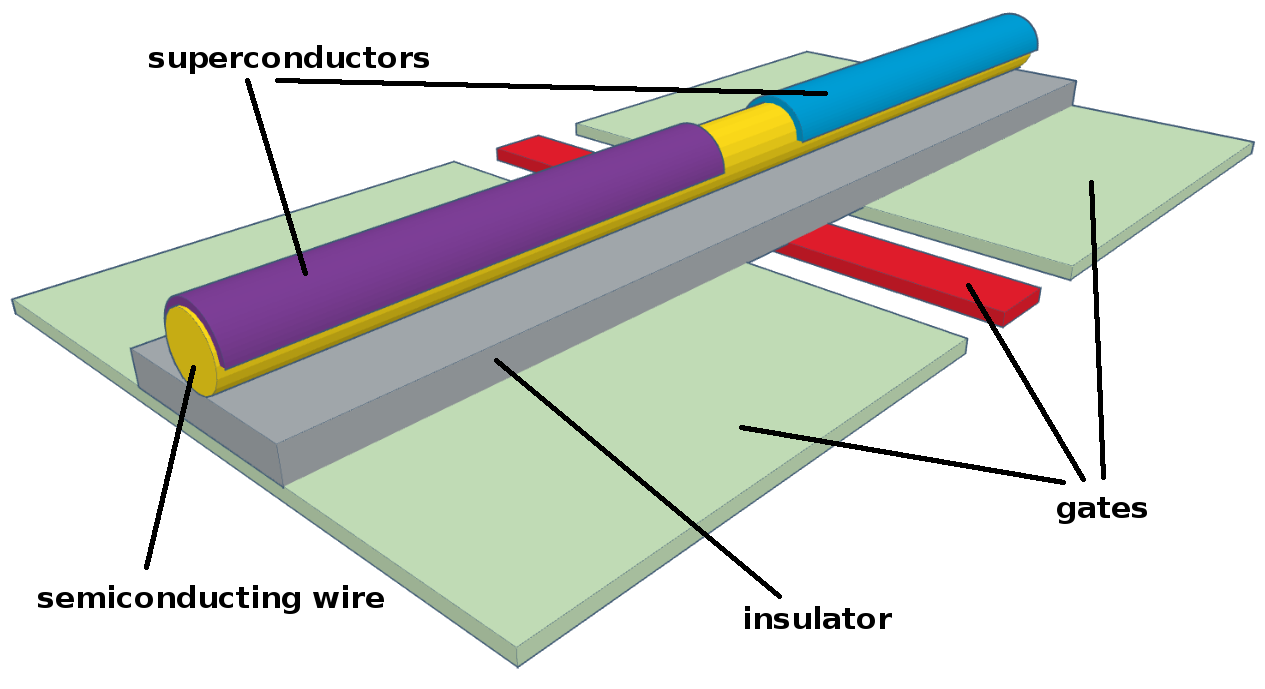
\includegraphics[width=0.7\linewidth]{images/real_model_3}
	\caption{Possible experimental realization of the system}
	\label{fig:realmodel3}
\end{figure}
The procedure of adjusting the parameters of the model from the chapter \ref{chap:model} can be the following: at first the system is created, with superconductivity order parameter inside the wires being as similar, as possible. This may require a really advanced technique of fabricating the samples. After that the magnetic field $ B $ is turned on and being adjust to be a little larger than $ \Delta $. After that the gates should be set to switch the wires to desired topology and create a tunnel barrier.

When the model was chosen, it was considered that it's much easier to make spatially inhomogeneous electric than magnetic field. It's also important, that the spin-orbit coupling energy inside the wire should be much stronger than the the superconducting gap. However, there is a hope that this condition can generally be satisfied, as the proximitized superconductivity can be weakened	 by a proper fabrication process.
\chapter{Conclusion}
\label{chap:conclision}
In this work we consider the system of two superconducting wires connected with a tunnel junction. A strong spin-orbit and a magnetic field perpendicular to the wire are assumed. The transparency of the barrier is set to be weak, so the system operates in tunneling regime. The model is introduced in detail in chapter \ref{chap:model}.

The low-energy spectrum is obtained for different topological indexes of the wires. The subgap states, found in section \ref{sec:Subgap_states}, are quite predictable.  In triv-top contact there is only one subgap state --- a Majorana state, on zero energy, as it should be. In top-top contact there are two subgap states, which are Majorana states, each from its own wire. As there is a finite transparency of the barrier, these states are not at zero energy and demonstrate the energy splitting, calculated in section \ref{subsect: weak_tunneling}. In triv-triv contact there are no subgape states --- this result, as well as the presence of only Majorana states in other contacts, wasn't obvious for us before, but also not especially surprising.

The supercurrent from low energy states is calculated in section \ref{sec:stationary_supercurrent}. The main result is that it is expected be much smaller than the current from high energy states and probably won't be observable.

In chapter \ref{chap:ionization} the model is modified by introducing time dependent perturbation. Even the simple case, when gap in the trivial wire is much smaller than the gap in topological one and the ionization amplitude factorizes, demonstrates a rich physics with four different subregimes. The ionization rates for Majorana state for these subregimes are calculated, as well as the limits of applicability and their physical meaning is established.

Authors hope, that this work can give further incites for both developing experimental techniques of detecting Majorana states in 1D superconductors and theoretical studies of properties of such systems.
\appendix
%\include{chapters/appa}
\chapter{Wavefunctions for the stationary contact}
\label{app:wavefunctions_with_corrections}

	Here the eigenstates of the junction are presented in leading and subleading order on the tunneling constant $ t $. Only long-wave ($ \wf{}{\medium} $ and $ \wf{}{\verylong} $) part is presented here, as it's sufficient for chapter \ref{chap:ionization}.	
	
	 The states in Nambu-Gorkov space are written in bra-ket notation. For zero tunneling they are:
  $ \big|\gamma_{0}\,\big> $--- the Majorana state and $ \big|\varepsilon,L_{0}\,\big> $, $ \big|\varepsilon,R_{0}\,\big> $ --- continuous spectra in the left and in the right wire respectfully.  The corrections are denoted as $ \big|\gamma_{1}\,\big> $, $ \big|\varepsilon,L_{1}\,\big> $, $ \big|\varepsilon,R_{1}\,\big> $. 
  
  It's important to note, that the first order correction for any state is located in the wire opposite to the one hosting the leading order. This can be reflected  with spinors in $ LR $-space as:  
\begin{gather}
\Psi_{\gamma}=\begin{pmatrix}0\\
\big|\gamma_{0}\,\big>
\end{pmatrix}_{LR}+\begin{pmatrix}\big|\gamma_{1}\,\big>\\
0
\end{pmatrix}_{LR}+...\\\Psi_{R}=\begin{pmatrix}0\\
\big|\varepsilon,R_{0}\,\big>
\end{pmatrix}_{LR}+\begin{pmatrix}\big|\varepsilon,R_{1}\,\big>\\
0
\end{pmatrix}_{LR}+...\\\Psi_{L}=\begin{pmatrix}\big|\varepsilon,L_{0}\,\big>\\
0
\end{pmatrix}_{LR}+\begin{pmatrix}0\\
\big|\varepsilon,L_{1}\,\big>
\end{pmatrix}_{LR}+...
\end{gather}


  The states are normalized as:
\begin{gather}
	\big\langle\gamma_{0}\big|\gamma_{0}\,\big>=1
	~~~~
	\big\langle\epsilon,R_{0}\,\big|\varepsilon,R_{0}\,\big>=N_{R}\left(\epsilon\right)\delta\left(\epsilon-\varepsilon\right)
	~~~~
	\big\langle\epsilon,L_{0}\,\big|\varepsilon,L_{0}\,\big>=N_{L}\left(\epsilon\right)\delta\left(\epsilon-\varepsilon\right)
\end{gather}
where
\begin{gather}
\label{N_L_N_R_definition}
	N_{L}\left(\varepsilon\right)=\frac{4\pi u\sqrt{\varepsilon^{2}-g_{L}^{2}}\left(e^{2\ensuremath{\kappa_{L}\left(\varepsilon\right)}}+1\right)^{2}}{\varepsilon}
	~~~~
	N_{R}\left(\varepsilon\right)=\frac{4\pi u\sqrt{\varepsilon^{2}-g_{R}^{2}}\left(e^{2\eta_{R}\left(\varepsilon\right)}+1\right)^{2}}{\varepsilon}
\end{gather}

Note, that for calculating $ s $-matrix another normalization, providing $ \bra{\epsilon} v \ket{\varepsilon} = \delta\br{\epsilon-\epsilon} $ should be used, with $ v=u\sigma_z\tau_z $ for long-wave states. The normalization used here serves for computing tunnel Hamiltonian matrix elements.

The definition of the $ \eta_{L,R} $, $ \eta_L $ and $ \kappa_R $ is given in the \ref{sec:stationary_supercurrent}. The indexes $ L,R $  near the spinors are relate to the wire, where this spinor is present. All the wavefucntions listed here  are relevant for both $ \abs{g_{L}}<g_{R} $ and $ \abs{g_{L}}>g_{R} $ cases.

The Majorana state is:
\begin{gather}
	\big<x\big|\gamma_{0}\,\big>=\frac{1}{2}\sqrt{\frac{g_{R}}{u}}\begin{pmatrix}-1\\
	i\\
	-i\\
	1
	\end{pmatrix}_{R}e^{-\frac{g_{R}x}{u}}
	\\
	\big<x\big|\gamma_{1}\,\big>=\frac{1}{2}\sqrt{\frac{g_{R}}{u}}\zeta t\left(e^{i\frac{\phi}{2}}+e^{-i\frac{\phi}{2}}\right)\left[\begin{pmatrix}-i\\
	1\\
	1\\
	-i
	\end{pmatrix}_{L}e^{-\frac{2\Delta x}{u}}-i\zeta\begin{pmatrix}-i\\
	-1\\
	1\\
	i
	\end{pmatrix}_{L}e^{-\frac{\left|g_{L}\right|x}{u}}\right]
\end{gather}

Continuous states from the right wire are:

\begin{multline}
	\big<x\big|E,\,R_{0}\big>=
	\\
	\left(-ie^{\eta_{R}\left(E\right)}-1\right)\begin{pmatrix}-1\\
	-e^{\eta_{R}\left(E\right)}\\
	e^{\eta_{R}\left(E\right)}\\
	1
	\end{pmatrix}_{R}e^{-\frac{ix\sqrt{E^{2}-g_{R}^{2}}}{u}}+\left(e^{\eta_{R}\left(E\right)}+i\right)\begin{pmatrix}-e^{\eta_{R}\left(E\right)}\\
	-1\\
	1\\
	e^{\eta_{R}\left(E\right)}
	\end{pmatrix}_{R}e^{\frac{ix\sqrt{E^{2}-g_{R}^{2}}}{u}}
\end{multline}
\begin{multline}
	\big<x\big|E\,R_{1}\big>\Big|_{E<g_{L}}=
	t\zeta\left(e^{2\eta_{R}\left(E\right)}-1\right)\left(e^{i\frac{\phi}{2}}+e^{-i\frac{\phi}{2}}\right)\times
	\\
	\times\left[\begin{pmatrix}-i\\
	1\\
	1\\
	-i
	\end{pmatrix}_{L}-e^{-\frac{2\Delta x}{u}}-\frac{2i\zeta}{\left(1+e^{-i\theta_{L}\left(E\right)}\right)}\begin{pmatrix}-ie^{-i\theta_{L}\left(E\right)}\\
	-1\\
	1\\
	ie^{-i\theta_{L}\left(E\right)}
	\end{pmatrix}_{L}e^{\frac{-x\sqrt{g_{L}^{2}-E^{2}}}{u}}\right]
\end{multline}
\begin{multline}
	\big<x\big|E\,R_{1}\big>\Big|_{E>g_{L}}=
	t\zeta\left(e^{2\eta_{R}\left(E\right)}-1\right)\left(e^{i\frac{\phi}{2}}+e^{-i\frac{\phi}{2}}\right)\times\\
	\times
	\left[\begin{pmatrix}-i\\
	1\\
	1\\
	-i
	\end{pmatrix}_{L}e^{-\frac{2\Delta x}{u}}-\frac{2i\zeta}{\left(1+ie^{-\kappa_{l}\left(E\right)}\right)}\begin{pmatrix}e^{-\kappa_{L}\left(E\right)}\\
	-1\\
	1\\
	-e^{-\kappa_{L}\left(E\right)}
	\end{pmatrix}_{L}e^{\frac{ix\sqrt{E^{2}-g_{L}^{2}}}{u}}\right]
\end{multline}
Continuous states from the left wire are:
\begin{multline}
	\big<x\big|\varepsilon,L_{0}\,\big>=\\\left(e^{\ensuremath{\kappa_{L}\left(\varepsilon\right)}}-i\right)\begin{pmatrix}1\\
	-e^{\ensuremath{\kappa_{L}\left(\varepsilon\right)}}\\
	e^{\ensuremath{\kappa_{L}\left(\varepsilon\right)}}\\
	-1
	\end{pmatrix}_{L}e^{+i\frac{\sqrt{\varepsilon^{2}-g_{L}^{2}}}{u}x}+\left(-1+ie^{\ensuremath{\kappa_{L}\left(\varepsilon\right)}}\right)\begin{pmatrix}e^{\ensuremath{\kappa_{L}\left(\varepsilon\right)}}\\
	-1\\
	1\\
	-e^{\ensuremath{\kappa_{L}\left(\varepsilon\right)}}
	\end{pmatrix}_{L}e^{-i\frac{\sqrt{\varepsilon^{2}-g_{L}^{2}}}{u}x}
\end{multline}
\begin{multline}
	\big<x\big|\varepsilon,L_{1}\,\big>\Big|_{\varepsilon<g_{R}}=
	\zeta t\left(e^{2\kappa_{L}\left(\varepsilon\right)}-1\right)\left(e^{i\frac{\phi}{2}}+e^{-i\frac{\phi}{2}}\right)
	\times
	\\
	\times
	\left[\frac{2i\zeta}{\left(-1+e^{i\theta_{R}\left(\varepsilon\right)}\right)}\begin{pmatrix}-1\\
	ie^{i\theta_{R}\left(\varepsilon\right)}\\
	-ie^{i\theta_{R}\left(\varepsilon\right)}\\
	1
	\end{pmatrix}_{R}e^{-x\frac{\sqrt{g_{r}^{2}-\varepsilon^{2}}}{u}}+\begin{pmatrix}1\\
	-i\\
	-i\\
	1
	\end{pmatrix}_{R}e^{-\frac{2\Delta x}{u}}\right]
\end{multline}
\begin{multline}
	\big<x\big|\varepsilon,L_{1}\,\big>\Big|_{\varepsilon>g_{R}}=\zeta t\left(e^{2\kappa_{L}\left(\varepsilon\right)}-1\right)\left(e^{i\frac{\phi}{2}}+e^{-i\frac{\phi}{2}}\right)\times\\\times\left[\frac{2it\zeta}{\left(-1+ie^{-\eta_{R}\left(\varepsilon\right)}\right)}\begin{pmatrix}-1\\
	-e^{-\eta_{R}\left(\varepsilon\right)}\\
	e^{-\eta_{R}\left(\varepsilon\right)}\\
	1
	\end{pmatrix}_{R}e^{\frac{ix\sqrt{E^{2}-g_{R}^{2}}}{u}}+\begin{pmatrix}1\\
	-i\\
	-i\\
	1
	\end{pmatrix}_{R}e^{-\frac{2\Delta x}{u}}\right]
\end{multline}
\chapter{Tunnel Hamiltonian derivation} 
\label{app:tunnel}
The goal in derivation tunnel Hamiltonian is to make it restoring the corrections of the wavefuncitons from appendix \ref{app:wavefunctions_with_corrections}.
Recalling, that in $ LR $-space the Hamiltonian has the form (\ref{tunnel_Hamiltonian_formalizm}), we write the unperturbed Green function as:
\begin{multline}
G_{0}\left(E\right)=\frac{1}{E+i0}\begin{pmatrix}0 & 0\\
0 & \big|\gamma_{0}\,\big>\big<\gamma_{0}\,\big|
\end{pmatrix}_{LR}+\int_{g_{L}}^{\infty}\frac{d\varepsilon}{N_{L}\left(\varepsilon\right)}\frac{1}{E+i0-\varepsilon}\begin{pmatrix}\big|\varepsilon,L_{0}\,\big>\big<\varepsilon,L_{0}\,\big| & 0\\
0 & 0
\end{pmatrix}_{LR}+\\+\int_{g_{l}}^{\infty}\frac{d\varepsilon}{N_{R}\left(\varepsilon\right)}\frac{1}{E+i0-\varepsilon}\begin{pmatrix}0 & 0\\
0 & \big|\varepsilon,R_{0}\,\big>\big<\varepsilon,R_{0}\,\big|
\end{pmatrix}_{LR}
\end{multline}
with $ N_{L,R} $ from (\ref{N_L_N_R_definition}). 
The corrections for the spinors should be calculated as:
\begin{gather}
\Psi_{1}\left(E\right)=G_{0}\left(E\right)H_{T}\Psi_{0}\left(E\right)
\end{gather}
So, for different states:
\begin{align}
\big|\gamma_{1}\,\big>&=\int_{g_{L}}^{\infty}\frac{d\varepsilon}{N_{L}\left(\varepsilon\right)}\,\frac{1}{-\varepsilon+i0}\big|\varepsilon,L_{0}\,\big>\,\big<\varepsilon,L_{0}\,\big|h_{LR}\big|\gamma_{0}\,\big>
\\
\big|E+i0,R_{1}\,\big>&=\int_{g_{L}}^{\infty}\frac{d\varepsilon}{N_{L}\left(\varepsilon\right)}\,\frac{1}{E-\varepsilon+i0}\big|\varepsilon,L_{0}\,\big>\,\big<\varepsilon,L_{0}\,\big|h_{LR}\big|E\,R_{0}\big>
\\
\nonumber
\big|E+i0,L_{1}\,\big>&=\frac{1}{E+i0}\big|\gamma_{0}\,\big>\,\big<\gamma_{0}\,\big|h_{LR}^{\dagger}\big|E,L_{0}\,\big>+
\\	
&\qquad\qquad\qquad\qquad
+\int_{g_{l}}^{\infty}\frac{d\varepsilon}{N_{R}\left(\varepsilon\right)}\,\frac{1}{E-\varepsilon+i0}\big|\varepsilon\,R_{0}\big>\,\big<\varepsilon,R_{0}\,\big|h_{LR}^{\dagger}\big|E,L_{0}\,\big>
\end{align}

Now, multiplying the third equation by $ \big<\gamma_{0}\,\big| $ and $ \big<\epsilon,R_{0}\,\big |$, find:
\begin{gather}
\big<\gamma_{0}\,\big|E+i0,L_{1}\,\big>=\frac{1}{E+i0}\,\big<\gamma_{0}\,\big|h_{LR}^{\dagger}\big|E,L_{0}\,\big>
\\
\big<\epsilon,R_{0}\,\big|E+i0,L_{1}\,\big>=\frac{1}{E-\epsilon+i0}\big<\epsilon,R_{0}\,\big|h_{LR}^{\dagger}\big|E,L_{0}\,\big>
\end{gather}

The l.h.s. of this equation can be calculated with the help of appendix \ref{app:wavefunctions_with_corrections}. After doing so, we arrive to the result (\ref{tunnel_matrix_elements_maj-cont}).
\chapter{Multiphoton ionization} 
\label{app:multiphoton ionization}
This appendix is focused on high-order perturbation theory, ionization rates in particular. 

\section{Basics about Green's functions}

The starting point is the general setup of a discrete bound state subject to a weak and slow perturbation $ V(t) $.The bound state energy is zero. The goal is to obtain the ionization rate. The time evolution of the wave function obeys the Schroedinger equation:
\begin{gather}
\label{shr_eq_general}
	i\frac{\partial}{\partial t}\Psi=(H_{0}+V)\Psi
\end{gather}

In the absence of perturbations, the solution is $ \Psi(t)=\Psi_{0} $ (since $ E_{0}=0 $ it is literally time-independent). For further analysis it's convenient to consider the unperturbed retarded Green's function $ G^{R}(E) $ defined so that:
\begin{gather}
\label{green_function_def}
	G^{R}(E)(E+i0-H_{0})=1
\end{gather}
If the bound state is normalized, $ \langle\gamma|\gamma\rangle= $1 and the continuous spectrum is normalized according to $ \langle E|E'\rangle=N(E)\delta(E-E') $ with some reasonably nice $ N(E $) then:
\begin{gather}
\mathbb{I}=|\gamma\rangle\langle\gamma|+\int\frac{|E\rangle\langle E|}{N(E)}dE
\end{gather}
Similarly, $ H_{0} $ and $ G^{R} $ in the energy representation:
\begin{gather}
	H_{0}=\int\frac{|E\rangle\langle E|}{N(E)}EdE
	\qquad
	G^{R}(\epsilon)=\frac{|\gamma\rangle\langle\gamma|}{\epsilon+i0}+\int\frac{|E\rangle\langle E|}{(\epsilon+i0-E)N(E)}dE
\end{gather}
Integrals over $ E $ include all states in the continuous spectrum. Where the latter is degenerate, a summation over the degenerate states must be carried out. From now on the "$ R $" index for retarded Green's function will be omitted.

In time representation the Green's function obeys:
\begin{gather}
	\left(i\frac{\partial}{\partial t_{2}}-H_{0}\right)G(t_{2},t_{1})=\delta(t_{2}-t_{1})
\end{gather}
One can formally introduce the Green's function in energy representation with two arguments as a Fourier-transform of $ G(t_{2},t_{1}) $:
\begin{gather}
	G\br{E_2,E_1}
	=
	\iint
	e^{iE_2t_2-iE_1t_1}
	G(t_{2},t_{1})
	dt_1
	dt_2
\end{gather}
As $ H_0 $ is time independent, $ G\br{t_2,t_1}=G\br{t_2-t_1,0} $, so:
\begin{gather}
	G\br{E_2,E_1}=2\pi \delta\br{E_2-E_1} G\br{E_1}
\end{gather}
One can also find, that for any eigenstate $ \ket{E_0} $
\begin{gather}
	G\br{t}\ket{E_0}
	=
	-ie^{-iE_0t}\theta_H\br{t}\ket{E_0}
\end{gather}
With the help of Green's function the Schroedinger equation (\ref{shr_eq_general}) can be solved as:
\begin{multline}
\label{general_expression_for the_wavefunction}
\Psi(t)=\Psi_{0}+\int G_{0}(t-t')V(t')\Psi_{0}(t')dt'+
\\
\iint G_{0}(t-t')V(t')G_{0}(t'-t'')V(t'')\Psi_{0}(t'')dt'dt''+\dots
\end{multline}
where the $ \Psi_0 $ is unperturbed wavefunction. This equation can be rewriteen  by the introducion 
\section{Fermi Golden Rule (first order)}

Consider first the lowest order to the Fermi Golden rule by only keeping the linear term in $ V $. Let the Fourier decomposition of $ V $ be:
\begin{gather}
\label{fourier_pertrubation}
	V(t)=\sum_n V_{n}e^{-i\omega_{n}t}
\end{gather}
(Hermiticity demands $ V(t)=V(t)^{*} $ so that $ V_{n}=V_{-n}^{*} $). Suppose there is an unperturbed continuous spectrum parameterized by $ E $, with $ \langle E|E'\rangle=f(E)\delta(E-E') $. The first step is to calculate $ \langle E|\Psi(t)\rangle $, i.e. the quantum amplitude of being in state $ |E\rangle $ at time $ t $. It is:
\begin{multline}
	\langle E|\Psi(t)\rangle=\langle E|\int G_{0}(t-t')V(t')\Psi_{0}(t')dt'\rangle=\int\langle E|G_{0}(t-t')V(t')|\Psi_{0}\rangle dt'=\\=\int\int\langle E|G_{0}(t-t')|E'\rangle\langle E'|V(t')|\Psi_{0}\rangle dt'\frac{dE'}{N(E)}
	\\=\int e^{-i(t-t')E}\theta_{H}(t-t')\langle E|V(t')|\Psi_{0}\rangle dt'=\\=e^{-iEt}\sum_{n}\int e^{it'(E-\omega_{n})}\theta_{H}(t-t')\langle E|V_{n}|\Psi_{0}\rangle dt'
\end{multline}

Assuming that the perturbation was turned on at $ t'=0 $ the integral over $ t' $ is taken from $ t_{0} $ to $ t $ and gives:
\begin{gather}
	\langle E|\Psi(t)\rangle=e^{-iEt}\sum_{n}\langle E|V_{n}|\Psi_{0}\rangle\frac{e^{it(E-\omega)}-1}{i(E-\omega_{n})}
\end{gather}

Thus, the probability density of being in the state $ |E\rangle $ is (omit all frequencies except the resonant on should be ommited since the contributions from non-resonant frequencies can be neglected at long times):
\begin{gather}
	\rho(E)=|\langle E|V_{n}|\Psi_{0}\rangle|^{2}\frac{4\sin^{2}\frac{t(E-\omega_{n})}{2}}{(E-\omega_{n})^{2}}
\end{gather}
so that the probability of being in a state between $ E $ and $ E+\delta E $ is at large times:

\begin{multline}
	P(E+\delta E,E)=|\langle E|V_{n}|\Psi_{0}\rangle|^{2}\intop_{E}^{E+\delta E}\frac{dE}{N(E)}\frac{4\sin^{2}\frac{t(E-\omega_{n})}{2}}{(E-\omega_{n})^{2}}=\\=2t|\langle E|V_{n}|\Psi_{0}\rangle|^{2}\intop_{E}^{E+\delta E}\frac{d(tE/2)}{N(E)}\frac{4\sin^{2}\frac{t(E-\omega_{n})}{2}}{t^{2}(E-\omega_{n})^{2}}=\\=2t|\langle E|V_{n}|\Psi_{0}\rangle|^{2}\frac{\pi}{N(E)}\theta_{H}(\omega_{n}-E)\theta_{H}(E+\delta E-\omega_{n})
\end{multline}
In other words, the probability density at large t behaves exactly like the $ \delta $-function:
\begin{gather}
	\rho(E)=2\pi|\langle E|V_{n}|\Psi_{0}\rangle|^{2}\delta(E-\omega_{n})
\end{gather} 
which is the well-known Fermi Golden rule. (Note, that the probability is $ dP=\rho(E)dE/f(E) $ – do not forget the normalization). Thus, the ionization rate (i.e. $ P/t $) for a single photon is expressed as:
\begin{gather}
\label{golden_reul_first_order}
	I=\frac{2\pi|\langle E|V_{n}|\Psi_{0}\rangle|^{2}}{f(E)}
\end{gather}
\section{Fermi Golden Rule (high order)}
Tho treat the higher-order perturbation theory it's convenient to rewrite (\ref{general_expression_for the_wavefunction}) as:
\begin{gather}
	\Psi(t)=\Psi_{0}+\int\int G_{0}(t-t')W(t',t'')\Psi_{0}(t'')dt'dt''
\end{gather}
where W incorporates all powers of perturbation theory:
\begin{gather}
	W=V+VG_0V+VG_0VG_0V+\dots
\end{gather}
The perturbation $ V $ in energy space is:
\begin{multline}
	V(E',E)\equiv\int V(t',t)e^{it'E'-iEt}dt'dt=\int V(t)e^{i(E'-E)t}dt=\\=\sum_{n}V_{n}\int e^{i(E'-E-\omega_{n})t}dt=\sum_{n}V_{n}2\pi\delta(E'-E-\omega_{n})
\end{multline}
The second term of the perturbation theory $ W_{2}=VGV $ in energy representation reads:
\begin{multline}
	W_{2}(E_{2},E_{1})=
	\int V(E_{2},E)G_0(E,E')V(E',E_{1})\frac{dEdE'}{(2\pi)^{2}}=
	\\
	\sum_{nm}2\pi\delta(E_{2}-E_{1}-\omega_{n}-\omega_{m})V_{n}G_{0}(E_{1}+\omega_{m})V_{m}
\end{multline} 
Very similarly, the $ N $-th-order term is:
\begin{gather}
	W_{N}(E_{2},E_{1})=\sum_{n_{1},\dots,n_{N}}2\pi\delta\left(E_{2}-E_{1}-\sum_{i=1}^{N}\omega_{n_{i}}\right)V_{n_{N}}\prod_{j=1}^{N-1}G_{0}\left(E_{1}+\sum_{s=1}^{j}\omega_{n_{s}}\right)V_{n_{j}}
\end{gather}

The above expression sums over all processes involving N photons. Note how the Green's functions contains the cumulative energy of all photons absorbed by the time. The $ \delta $-function at the start of the expression indicates that the energy is changed by $ \sum\omega_{n_{i}} $. It makes more sense to sort processes within $ W $ not by photon count $ N $ but rather by the total energy gained, since the total ionization rate should be dominated by ionization to the lowest accessible continuum state. Defining this activation energy as $ \mathcal{E} $, write:
\begin{gather}
W_{\mathcal{E}}(E_{2},E_{1})=2\pi\delta(E_{2}-E_{1}-\mathcal{E})w_{\mathcal{E}}(E_{1})\\
\label{ionization_key}
w_{\mathcal{E}}(E)
=
\sum_{\{n_{i}\}:\mathcal{E}}V_{n_{N}}\prod_{j=1}^{N-1}G_{0}\left(E+\sum_{s=1}^{j}\omega_{n_{s}}\right)V_{n_{j}}
\end{gather}
The summation is over all sets of photons $ {n_{i}} $ that total an energy of $ \mathcal{E} $, i.e. such sets that $ \sum_{i}^{N}\omega_{n_{i}}=\mathcal{E} $. The photon number N itself depends on the particular photon set $ n_{i} $. The total composite perturbation $ W $ can be written as a sum of $ W_{\mathcal{E}} $ with different $ \mathcal{E} $. However, only one term is relevant --- the one with $ \mathcal{E}=\min{|g_{L}|,|g_{L}| }$. (If the elementary frequency quantum $ \omega $ is large enough, this is replaced by the lowest $ \mathcal{E} $ that surpasses the minimum gap). 

Now  the Fermi Golden rule result (\ref{golden_reul_first_order}) can be rederived 	for $ W_{\mathcal{E}} $. It's easy ti see that $ W $ has the same energy structure as the single-photon perturbation $ V $. Both operators simply shift the energy. Thus, one may simply put $ W_{\mathcal{E}} $ into the Fermi Golden rule instead of $ V $ to get the full-theory results:
\begin{gather}
	I=\frac{2\pi|\langle\mathcal{E}|w_{\mathcal{E}}|\Psi_{0}\rangle|^{2}}{N(\mathcal{E})}
\end{gather}
Thus to find the ionization rate one should calculate $ w_{\mathcal{E}} $ from (\ref{ionization_key}).
%\bibliographystyle{siam}
%\bibliographystyle{plain}
\bibliography{main.bib}


\printbibliography
\end{document}

